\newacronym{jvm}{JVM}{Java Virtual Machine}
\newacronym{rest}{ReST}{Representational State Transfer}
\newacronym{dx}{DX}{Developer Experience}
\newacronym{vcs}{VCS}{Version Control System}
\newacronym{scm}{SCM}{Source Code Management}
\newacronym{fs}{FS}{File System}
\newacronym{ci}{CI}{Continuous Integration}
\newacronym{saas}{SaaS}{Software as a Service}
\newacronym{rdd}{RDD}{Resilient Distributed Dataset}
\newacronym{soc}{SoC}{Separation of Concerns}
\newacronym{dom}{DOM}{Document Object Model}
\newacronym{spa}{SPA}{Single Page Application}
\newacronym{seo}{SEO}{Search Engine Optimization}
\newacronym{hmr}{HMR}{Hot Module Replacement}
\newacronym{svg}{SVG}{Scalable Vector Graphics}
\newacronym{tf-idf}{TF-IDF}{Term Frequency -- Inverse Document Frequency}
\newacronym{utc}{UTC}{Coordinated Universal Time}
\newacronym{gmt}{GMT}{Greenwich Mean Time}


\section{Requirements Analysis}

This is a vital part and first step of our methodology leading to a proposed solution.


\subsection{UX Personas}

In order to derive a meaningful list of design\index{design} requirements we make use of an instrument from designing\index{design} products called \gls{ux} personas.

It has been pioneered for usage with software development by Cooper~\cite{Cooper2004}. The basic idea is to come up with some stereotypical ``personalities'' described by certain characteristics which represent our target user groups.
An important aspect is the potential creation of empathy with our future users.

Each of these personas is, typically, illustrated with a profile picture and at least a firstname.
The notion is to create some degree of familiarity and identifiability for the \gls{ux} designer\index{design} and other parties involved in the design\index{design} process.
Furthermore, usually, a persona is equipped with some demographical coordinates, some sort of tagline which serves as an executive summary, enhanced with background info, and motivations.
All of this information is normally pointed and rather skimped.
It should support in easily creating a vivid idea and image of the different users of the product in design\index{design}.

Finally, scenarios or user stories briefly describe ways in which these particular user types would use the imaginary product.
In the end, it is important the resulting personas can also be physically tangible -- for instance, printed out on cards and pinned onto a whiteboard.
Personas are a valuable tool for subsequent design\index{design} of \gls{ui} and interactions.

Table~\ref{tab:ux-personas} provides a high-level overview of the personas we came up with for our prototypical\index{prototype} software, focusing on skill set distribution.
As one can see, persona skills range from overall highly to overall lowly skilled as well as individuals with focus on certain different skills.
This makes for an interesting foundation as, all in all, quite a disperse set of potential users has to be catered for. The following pages contain our personas themselves.
The profile pictures were created with an online avatar tool\footnote{\textcolor{blue}{\href{http://avachara.com/avatar/}{avachara.com/avatar/}}}.

\begin{table}
  \centering
  \begin{tabular}{ccccccc}
    \toprule
    \emph{Skills}      & Hugo             & Alice          & Bob              & John    & Jane           & Walter  \\
    \midrule
    Technical          & \textbf{low}  & \textbf{high}  & low              & low     & high           & low     \\
    Scientific         & medium        & \textbf{high}  & \textbf{low}     & medium  & high           & high    \\
    Data-Related       & medium        & high           & \textbf{medium}  & medium  & \textbf{high}  & medium  \\
    Temporal Interest  & medium        & high           & \textbf{low}     & high    & \textbf{high}  & high  \\
    \bottomrule
  \end{tabular}
  \caption{UX personas skill summary and comparison. Edge entries in \textbf{bold}.}
  \label{tab:ux-personas}
\end{table}

\subsection{Requirements List} \label{sec:requirements-list}

Through the creation of our personas we were able to properly visualize and dissect corresponding requirements for our prototype\index{prototype}.
Consequently, we have derived these:

\begin{itemize}
  \item \textbf{R1:} The prototype\index{prototype} must be capable of loading and working with diverse datasets
  \item \textbf{R2:} Moreover, it must be intuitive for casual users (i.e., less technically expertized)
  \item \textbf{R3:} Yet, some shortcuts for rather power users should be supported as well
  \item \textbf{R4:} Focus of our approach\index{approach} has to be on visual-interactive\index{visual-interactive} charting aid
  \item \textbf{R5:} These charts must be centered on applying time-oriented\index{time-oriented} data transformations\index{transformation}
  \item \textbf{R6:} Plus, they should provide extraordinary visual overview of the dataset at hand
  \item \textbf{R7:} Thus, focus has to be put on choosing most effective and efficient visualizations
  \item \textbf{R8:} Furthermore, interactively exploring data must be conveniently possible
  \item \textbf{R9:} A more traditional tabular editor should be available with direct manipulation
  \item \textbf{R10:} Editing time-oriented\index{time-oriented} data should be supported by specific \gls{ui} controls
  \item \textbf{R11:} Data quality issues need to be easily identifiable and effectually addressable
  \item \textbf{R12:} Conveniently spotting data anomalies respectively outliers should be possible
  \item \textbf{R13:} Concrete time-oriented\index{time-oriented} data transformation\index{transformation} operations to be supported:
  \begin{itemize}
    \item Data cleaning regarding missing and erroneous values
    \item Normalization concerning points in time and intervals
    \item Merging columns in an intuitive visual-interactive\index{visual-interactive} way
    \item Formatting cleanup, e.g., inconsistencies or conversion
  \end{itemize}
\end{itemize}


\subsection{Hugo}


\includegraphics[scale=0.5]{figures/requirements/persona-avatar-hugo}

\subsubsection{Demographics}

\begin{itemize}
    \item Age: 35
    \item Location: Vienna, Austria
    \item Job: Business Analyst
    \item Expertise: Marketing \& Statistics\index{statistics}
\end{itemize}

\subsubsection{Tagline}

\textit{``I need to quickly filter out erroneous data from market survey results.''}

\subsubsection{Background}

\begin{itemize}
    \item Studied business administration focusing on marketing and specializing in statistics\index{statistics}
    \item Some years of working experience in the industry
    \item Responsible for pointing out business opportunities through analyses\index{analysis}
\end{itemize}

\subsubsection{Motivations}

\begin{itemize}
    \item Wants to see the ``big picture''
    \item Doesn't want to ``lose'' any time
\end{itemize}

\subsubsection{Scenarios (User Stories)}

\begin{itemize}
    \item Got huge amounts of messy real-world data from various market surveys
    \item Wants to ``scan'' this data quickly for using it in market/business analyses\index{analysis}
    \item Often data is time-oriented\index{time-oriented}, as it denotes market-related developments over time
\end{itemize}


\subsection{Alice}

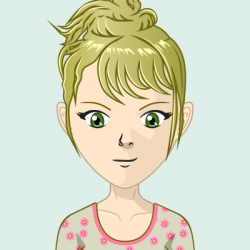
\includegraphics[scale=0.5]{figures/requirements/persona-avatar-alice}

\subsubsection{Demographics}

\begin{itemize}
    \item Age: 31
    \item Location: Vienna, Austria
    \item Job: Academic Researcher
    \item Expertise: Mathematics \& Statistics\index{statistics}
\end{itemize}

\subsubsection{Tagline}

\textit{``I'm interested in spending less time wrangling\index{wrangle} datasets suitable for analysis\index{analysis}.''}

\subsubsection{Background}

\begin{itemize}
    \item Studied mathematics with a focus on statistics\index{statistics} resulting in a research position in the field (post-doctoral)
    \item Special focus of the research group is time-oriented\index{time-oriented} data, being involved in various international projects
\end{itemize}

\subsubsection{Motivations}

\begin{itemize}
    \item Wants to analyze huge datasets, often containing flawed data
    \item She would rather spend time on analysis\index{analysis} than preparation
\end{itemize}

\subsubsection{Scenarios (User Stories)}

\begin{itemize}
    \item Got various sample time-oriented\index{time-oriented} datasets and wants to analyze the data
    \item Furthermore, wrangling\index{wrangle} should take less effort to apply Occam's razor
\end{itemize}


\subsection{Bob}

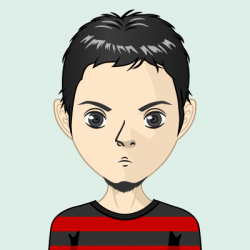
\includegraphics[scale=0.5]{figures/requirements/persona-avatar-bob}

\subsubsection{Demographics}

\begin{itemize}
    \item Age: 34
    \item Location: Graz, Austria
    \item Job: Journalist
    \item Expertise: Journalism \& Politics
\end{itemize}

\subsubsection{Tagline}

\textit{``I would like to be able to handle messy data for analysis\index{analysis} to be used in my articles.''}

\subsubsection{Background}

\begin{itemize}
    \item Graduate of communication studies with a specialization in politics
    \item Worked for several online news agencies
\end{itemize}

\subsubsection{Motivations}

\begin{itemize}
    \item Is held back from doing real ``data journalism'' due to lack of technical skills
    \item Would get into this kind of journalism if tools were better suited to his needs
\end{itemize}

\subsubsection{Scenarios (User Stories)}

\begin{itemize}
    \item Got an idea for a current news story based on some quite untidy political/economic data which is often of time-oriented\index{time-oriented} nature
    \item Is able to conveniently verify justification of story based on respective analysis\index{analysis} of wrangled\index{wrangle} data
\end{itemize}


\subsection{John}

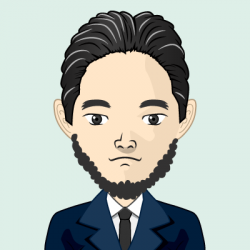
\includegraphics[scale=0.5]{figures/requirements/persona-avatar-john}

\subsubsection{Demographics}

\begin{itemize}
    \item Age: 40
    \item Location: Salzburg, Austria
    \item Job: Political Analyst
    \item Expertise: Politics \& Statistics\index{statistics}
\end{itemize}

\subsubsection{Tagline}

\textit{``I want to conveniently and visually prepare vast amounts of public poll data for analysis\index{analysis}.''}

\subsubsection{Background}

\begin{itemize}
    \item Studied political sciences with a focus on statistics\index{statistics} (Ph.D.)
    \item Works for news agencies, especially analyzing electoral situations
\end{itemize}

\subsubsection{Motivations}

\begin{itemize}
    \item Strong need to be able to get lots of data from various polls into unified schema with as little hassle as possible
    \item Is not particularly technically skilled or interested, just wants to get the data to be able analyzing it
\end{itemize}

\subsubsection{Scenarios (User Stories)}

\begin{itemize}
    \item Electoral poll data, consequently, mainly temporal natured, from various sources needs to get prepared respectively unified for analyzing
    \item Uses the visual-interactive\index{visual-interactive} tool being able to get the job done in a convenient way
\end{itemize}


\subsection{Jane}


\includegraphics[scale=0.5]{figures/requirements/persona-avatar-jane}

\subsubsection{Demographics}

\begin{itemize}
    \item Age: 37
    \item Location: Munich, Germany
    \item Job: Industrial Researcher
    \item Expertise: Biology \& Statistics\index{statistics}
\end{itemize}

\subsubsection{Tagline}

\textit{``I need a quick(er) and more reliable way to experiment with biological test data.''}

\subsubsection{Background}

\begin{itemize}
    \item Graduated in bio engineering
    \item Works at a pharmaceutical company testing new ways of synthesizing cosmetics
\end{itemize}

\subsubsection{Motivations}

\begin{itemize}
    \item Currently, the whole roundtrip of setting up test labs and analyzing results is cumbersome and takes much time
    \item Wants to be able to iterate in a quicker mode of operation by improving on wrangling\index{wrangle} test data applicable for actual analysis\index{analysis}
\end{itemize}

\subsubsection{Scenarios (User Stories)}

\begin{itemize}
    \item Is able to reduce testing roundtrips by using the visual-interactive\index{visual-interactive} tool for making time series test data useful for analysis\index{analysis}
    \item Based on experience and results from previous iterations she is able to decrease overall throughput time even more
\end{itemize}


\subsection{Walter}

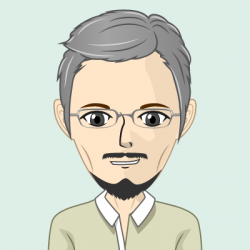
\includegraphics[scale=0.5]{figures/requirements/persona-avatar-walter}

\subsubsection{Demographics}

\begin{itemize}
    \item Age: 46
    \item Location: Vienna, Austria
    \item Job: Medical Doctor
    \item Expertise: Diabetes
\end{itemize}

\subsubsection{Tagline}

\textit{``I want to be able to conveniently visualize temporal therapy data provided by patients.''}

\subsubsection{Background}

\begin{itemize}
    \item Studied medicine, graduating cum laude
    \item Works at special center focusing on diabetics treatment
\end{itemize}

\subsubsection{Motivations}

\begin{itemize}
    \item Often, therapy data provided by patients is rather messy, that is, concerning missing respectively erroneous values, formatting, ...
    \item Wants to be able to visualize data to get to see the ``real'' picture
\end{itemize}

\subsubsection{Scenarios (User Stories)}

\begin{itemize}
    \item Using the tool he is able to reduce time spent on getting time-series-based therapy data provided by his patients ready for analysis\index{analysis} and can focus on actually analyzing
    \item Might even encourage (at least some of) his patients to use the tool themselves to further reduce overhead
\end{itemize}


\section{Design of UI and Interactions}

For designing\index{design} the \gls{ui} and interactions we have created mockups a.k.a. wireframes~\cite{Garrett2011}.

\subsection{UI Mockups}

The design\index{design} of our prototype\index{prototype} should meet our list of requirements. To this end, we created a number of mockups to be able to easily refine our designs\index{design}.

We have created our \gls{ui} mockups using \emph{Balsamiq\footnote{\textcolor{blue}{\href{https://balsamiq.com/}{balsamiq.com}}}} as productive tool.
An important aspect of wireframing is that it should be convenient creating the mockups.
One needs to be able to quickly iterate on ideas and throw away things which did not lead into the right direction.
Often, simply pencil and paper are being used which is already a good way to get to some first scribbles.
A quite common mistake is to skip proper wireframing and jump to design\index{design} screens immediately.
Most of the power within the creative design\index{design} process and flow is lost this way as design\index{design} screens take considerably more effort in producing them.
Consequently, iterating on these is usually more sluggish and throwing results away rather avoided.

The following pages contain our resulting wireframed mockups including some descriptions and further explanations regarding their functionality and respective underlying reasoning.
Mockups were created iteratively and evaluated in qualitative feedback loops until satisfying results have been achieved, that went into prototypical\index{prototype} implementation.

\subsubsection{Design Process}

While iteratively designing\index{design} with the help of mockups we constantly refined our ideas, adapting our approach\index{approach}, and trashing things that did not work out as expected.\\
Some material thereby discovered and/or changed:

\begin{itemize}
  \item Foremost, pie charts are, mostly, not useful in our context of transforming time-oriented\index{time-oriented} data
  \item On the other hand, bar charts are well suited to communicate quantities (e.g., of different table entries)
  \item Line charts, as commonly used for time series data, are not being emphasized on in our approach\index{approach}, mainly since we have found calendar heatmap visualizations to be superior for our use case, as our approach is generally not constrained to time series data but should be suitable for any time-oriented data
  \item Normalization functionality consciously left rather vague, to be fleshed out when actually developing the prototype\index{prototype}
  \item Modal dialogs containing interactive charts make sense for certain actions
  \item Visualizing the context of two different columns next to each other for exploratory comparison is beneficial
  \item A browser-based application is sufficient and a dedicated desktop one not needed in this case
\end{itemize}


\subsubsection{Upload Dialog}

\begin{figure}[h]
  \centering
  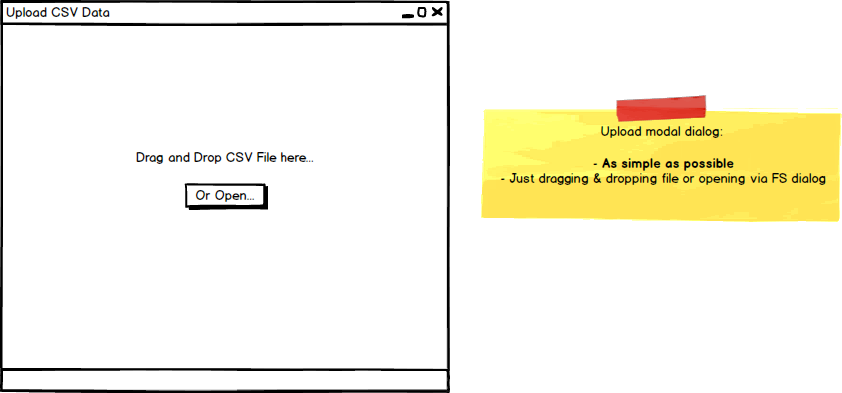
\includegraphics[width=1.125\textwidth]{figures/design/mockup-0}
  \caption{UI mockup of the upload dialog.}
  \label{fig:mockup-0}
\end{figure}

Naturally, the first \gls{ui} component we have designed\index{design} is the one which feeds the application with data to operate on:
the upload dialog (see Figure~\ref{fig:mockup-0}).

\begin{itemize}
  \item \textbf{Description}
  \begin{itemize}
    \item The main goal here was simplicity
    \item Consequently, truly simple dialog
    \item An area for dropping off file
  \end{itemize}
  \item \textbf{Reasoning}
  \begin{itemize}
    \item As it is central to the application, uploading has to be really simple
    \item Thus, with as little effort as possible
    \item That is, affordance has to be intuitive
  \end{itemize}
\end{itemize}

The idea regarding interaction is that as soon as a file is selected, the upload commences automatically, giving visual feedback of its progress to the user via according animation effects, disappearing as soon as it is finished.


\subsubsection{Table Editor}

\begin{figure}[h]
  \centering
  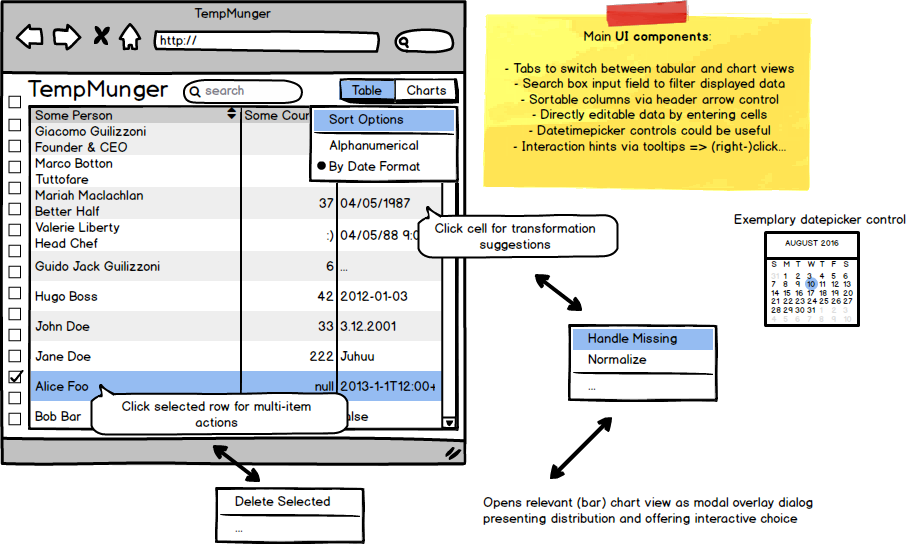
\includegraphics[width=1.2\textwidth]{figures/design/mockup-1}
  \caption{UI mockup of the table editor.}
  \label{fig:mockup-1}
\end{figure}

The table editor page (see Figure~\ref{fig:mockup-1}) has been designed\index{design} to be one of the two main pages of the application, the charts page being the second one, intuitively accessible via tabbed navigation in the upper right of the screen.

\begin{itemize}
  \item \textbf{Description}
  \begin{itemize}
    \item Enables direct manipulation editing of data
    \item Supports multi-row actions via check box selection
    \item Various search, sorting, and filtering options are available
    \item Provides menu access to further and more specialized dialogs
  \end{itemize}
  \item \textbf{Reasoning}
  \begin{itemize}
    \item The table editor is a well-known \gls{ui} metaphor for this use case
    \item Many users are familiar with editing tabular data from MS Excel \& co.
    \item It supplies the user with a straightforward and efficient mode of interaction
  \end{itemize}
\end{itemize}


\subsubsection{Missing Values Dialog}

\begin{figure}[h]
  \centering
  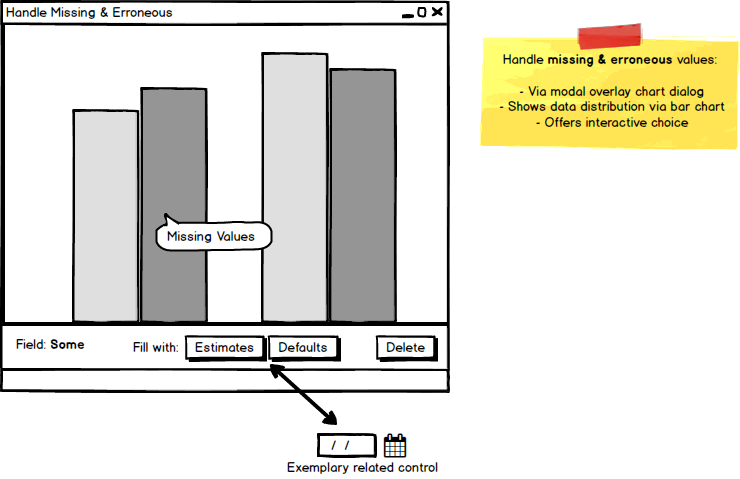
\includegraphics[width=1.12\textwidth]{figures/design/mockup-2}
  \caption{UI mockup of the missing values dialog.}
  \label{fig:mockup-2}
\end{figure}

The missing values dialog (see Figure~\ref{fig:mockup-2}) has been designed\index{design} to be opened from the table editor page via according menu access.

\begin{itemize}
  \item \textbf{Description}
  \begin{itemize}
    \item Concrete shape of chart not 100\% clear at this point
    \item Most probably, bar chart -- possibly, a horizontal one
    \item User is able to fill missing value entries or delete them
    \item Options provided are filling them with estimates or defaults
  \end{itemize}
  \item \textbf{Reasoning}
  \begin{itemize}
    \item Bar charts are capable of communicating distributions well
    \item Another possibility would be pie charts, but they are proven to be misleading
    \item To quote Tufte~\cite{Tufte2001}, p. 178: \emph{``Given
  their low density and failure to order numbers along a
  visual dimension, \textbf{pie charts should never be used}.''}\footnote{Cf. \textcolor{blue}{\href{https://www.edwardtufte.com/bboard/q-and-a-fetch-msg?msg\_id=00018S}{www.edwardtufte.com/bboard/q-and-a-fetch-msg?msg\_id=00018S}}}
  \end{itemize}
\end{itemize}


\subsubsection{Normalization Dialog}

\begin{figure}[h]
  \centering
  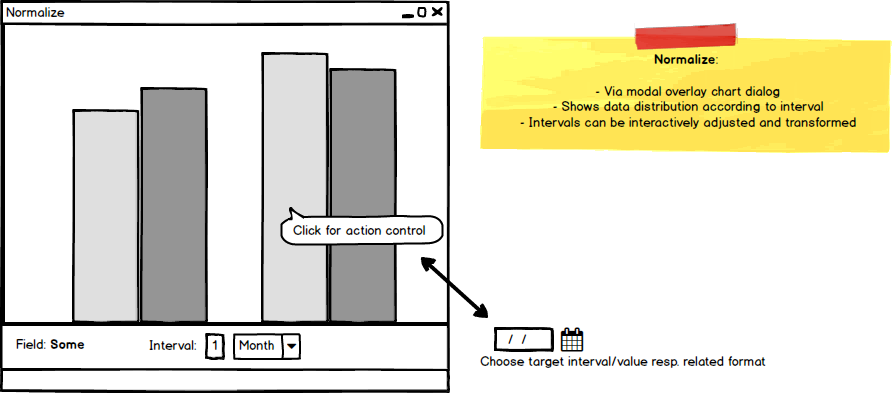
\includegraphics[width=1.2\textwidth]{figures/design/mockup-3}
  \caption{UI mockup of the normalization dialog.}
  \label{fig:mockup-3}
\end{figure}

The interval-focused normalization dialog (see Figure~\ref{fig:mockup-3}) is meant to be accessible via menu from the table editor page, too.

\begin{itemize}
  \item \textbf{Description}
  \begin{itemize}
    \item Its purpose is supposed to be enabling a user to normalize temporal intervals
    \item For batch-wise transforming\index{transformation} values of entries within a certain timespan
    \item Chart visualization is rather unclear at this stage
    \item Probably, bar chart as well -- but rather vertical one
    \item Interaction via point and click, including with chart
  \end{itemize}
  \item \textbf{Reasoning}
  \begin{itemize}
    \item The use case being worth covering became evident while gathering requirements
    \item Consequently, we will experiment with supporting it via meaningful interactive chart visualization
    \item Concrete characteristics will be shaped while iterative development itself
    \item Most probably, our color scheme of the chart visualization will be within neutral, plain gray to black range
    \item Since explicit coloring should only be used when it can communicate and, hence, convey meaning to the user, being intention-revealing, that is
    \item So, in the case of Figure~\ref{fig:mockup-2} it may make sense to use a noticeable color
  \end{itemize}
\end{itemize}


\subsubsection{Outlier Detection Alerting}

\begin{figure}[h]
  \centering
  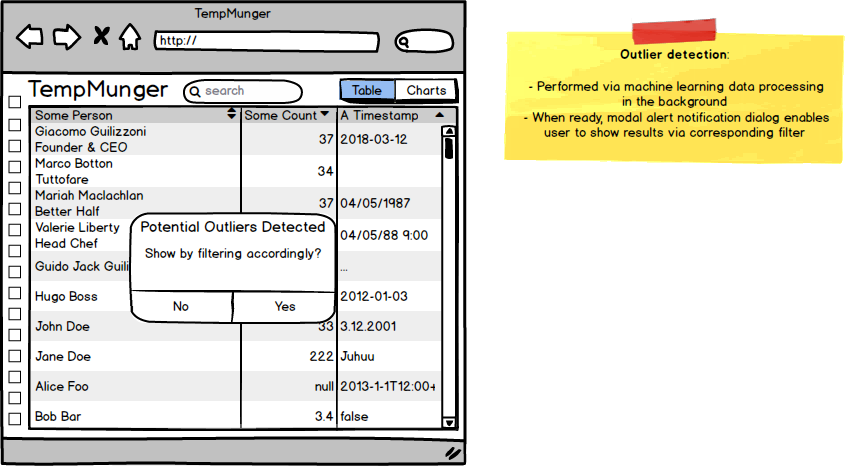
\includegraphics[width=1.1\textwidth]{figures/design/mockup-4}
  \caption{UI mockup of the outlier detection info alert.}
  \label{fig:mockup-4}
\end{figure}

When outliers are detected we need to show that to the user (see Figure~\ref{fig:mockup-4}).
As we intend to apply \glslink{ml}{machine learning} for this purpose, we need some way to do so without sacrificing good \gls{ux}.

\begin{itemize}
  \item \textbf{Description}
  \begin{itemize}
    \item Therefore, a simple modal dialog overlay is chosen
    \item It offers the user to display detected potential outliers
    \item When the user accepts, views are filtered accordingly
  \end{itemize}
  \item \textbf{Reasoning}
  \begin{itemize}
    \item Corresponding \gls{ml} processing has to happen in the background
    \item This is due to its potentially longer lasting computation time
    \item Consequently, informing the user about results has to be as unobtrusive as possible without interruption
    \item So, it should definitely not interfere with the current workflow, goals, and tasks of the user
    \item Thus, we intend to make use of an overlay which does not block the \gls{ui} and stays around for later use, more like an interactive notification-style message
  \end{itemize}
\end{itemize}


\subsubsection{Table Column Merging}

\begin{figure}[h]
  \centering
  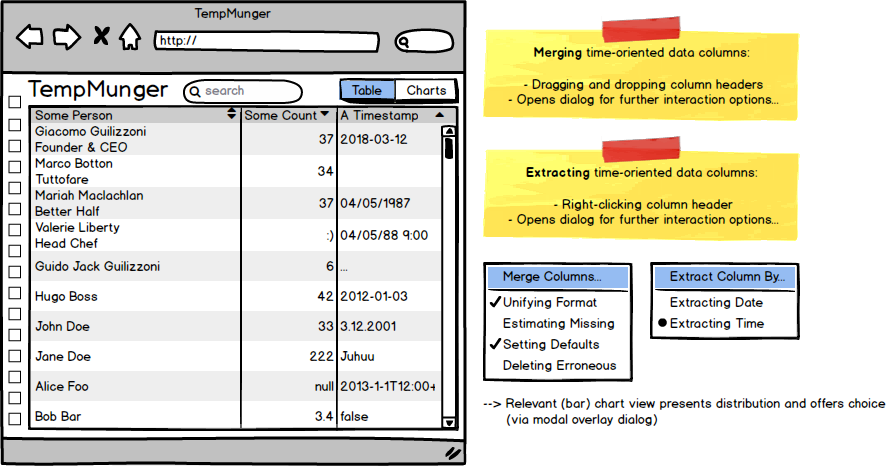
\includegraphics[width=1.175\textwidth]{figures/design/mockup-5}
  \caption{UI mockup of merging table columns via drag \& drop.}
  \label{fig:mockup-5}
\end{figure}

An interesting idea is to enable merging time-oriented\index{time-oriented} data columns via drag \& drop interaction metaphor (see Figure~\ref{fig:mockup-5}).

\begin{itemize}
  \item \textbf{Description}
  \begin{itemize}
    \item So when dragging a temporal column unto another, a related merging operation should be initiated
    \item The initial idea is to offer optional choice regarding the merge via a menu then
    \item Options like what to do with missing values and how to merge values in general
    \item Another idea is enabling column extraction via drag \& drop as well, still somewhat vague, though
  \end{itemize}
  \item \textbf{Reasoning}
  \begin{itemize}
    \item Many users are familiar with the basic kind of this interaction from spreadsheet applications like Excel
    \item Consequently, when indicating via according cursor on hover it is likely users will give it a spin
    \item Corresponding coloring of drop targets while dragging would be helpful to support the user with the interaction
  \end{itemize}
\end{itemize}


\subsubsection{Charts Page}

\begin{figure}[h]
  \centering
  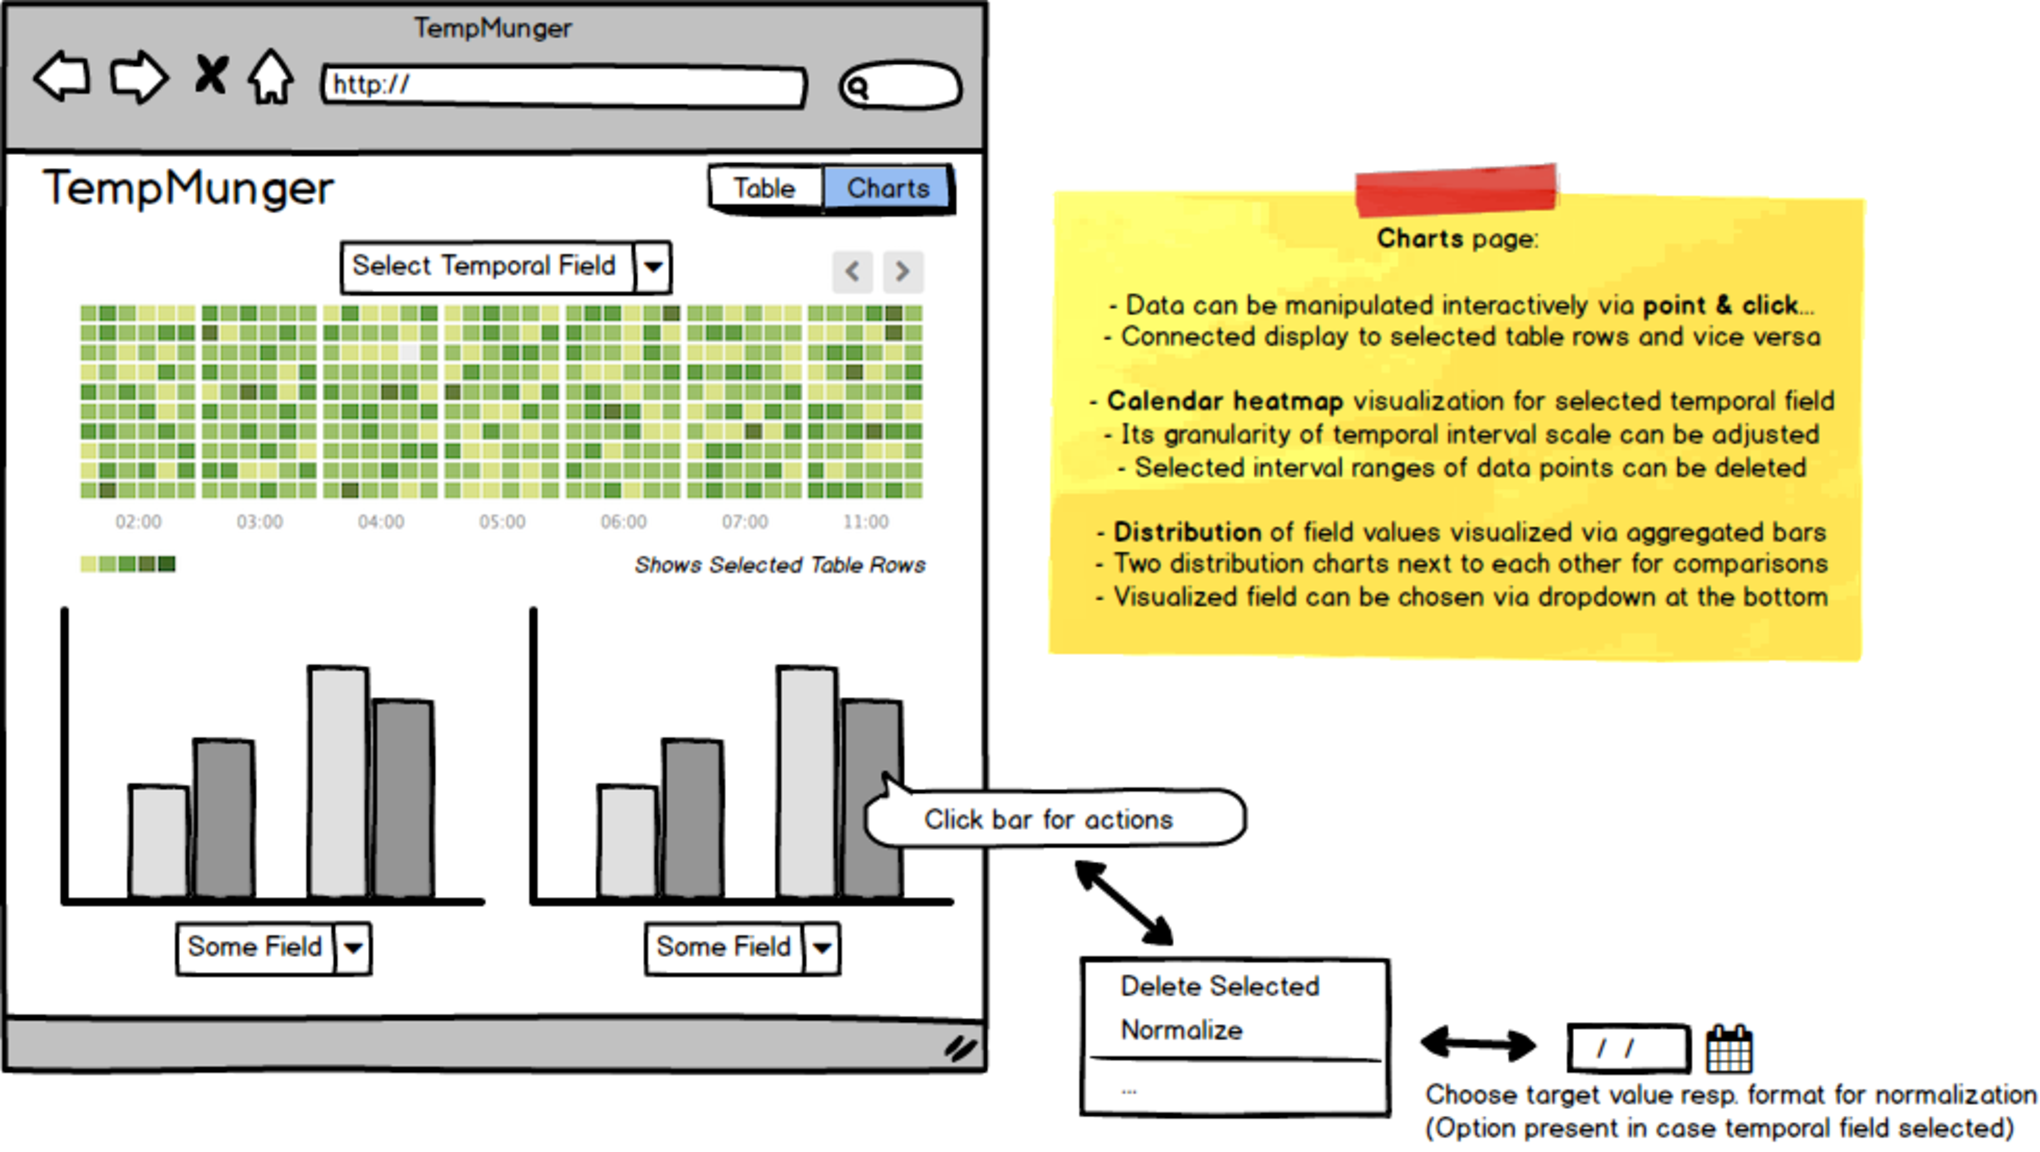
\includegraphics[width=1.1\textwidth]{figures/design/mockup-6}
  \caption{UI mockup of the charts page including calendar heatmap visualization.}
  \label{fig:mockup-6}
\end{figure}

The charts page is the second of the two main pages of the application, next to the initial table editor one.

\begin{itemize}
  \item \textbf{Description}
  \begin{itemize}
    \item It is headed by an interactive calendar heatmap visualization
    \item Below, two distribution bar charts are next to each other
    \item Controls allow interacting with the charts, plus their items should be interactive
    \item Table editor filtering is intended to be interconnected with charts page views
  \end{itemize}
  \item \textbf{Reasoning}
  \begin{itemize}
    \item Calendar heatmap visualizations are particularly useful for displaying time-oriented\index{time-oriented} data distributions
    \item Densities of data therein are usually visualized via appropriate color scheming, popularly ranging in the green spectrum
    \item Histogram-like bar charts are useful for viewing data distributions in general
    \item Having two of the latter next to each other is great for comparisons, interactive exploration, and discovery
  \end{itemize}
\end{itemize}


\section{Iterative Prototyping}

Following the creation of our \gls{ui} mockups and agreeing that a satisfiable state had been reached, we started with implementing the corresponding prototypical\index{prototype} software.

So, we developed in an agile manner, meaning close contact and collaboration with the ``client'', in this case the assisting thesis advisor.
Plus, developing respective parts of the application iteratively, chunk by chunk, preferably with short iteration cycles.
While developing new features there were also regular short phases in between, where focus was laid on bug fixing, cleanup, and polishing of existing things.

Therefore, we have set up a live testing environment, easily accessible for the client, regularly shipping changes, and gathering feedback to be incorporated as promptly as possible.
Technical details regarding the setup are described in Appendix~\ref{ch:appendix-a}.

As workflows in this project were particularly lean and lightweight, no special issue management software was used.
It generally sufficed to make use of simple tools like \emph{Wunderlist}\footnote{\textcolor{blue}{\href{https://www.wunderlist.com/}{www.wunderlist.com}}}, \emph{Simplenote}\footnote{\textcolor{blue}{\href{https://simplenote.com/}{simplenote.com}}}, and email communication for tracking, planning as well as discussing todos, tasks, and issues.
Additionally, from time to time when felt necessary and considered potentially fruitful, personal meetings were held.
Mainly for hands-on demoing and reviewing purposes, plus, talking about direction-giving decisions.

This process was followed until the prototype\index{prototype} eventually reached feature-completeness.


\section{TempMunger}

This section goes into some details regarding the implemented prototype\index{prototype} itself.
Extensive documentation of related software design\index{design} and architecture\index{architecture} can be found in Appendix~\ref{ch:appendix-a}.


\subsection{Implementation Details}

As \gls{ide}, \emph{IntelliJ IDEA\footnote{\textcolor{blue}{\href{https://www.jetbrains.com/idea/}{www.jetbrains.com/idea/}}}} was used. \\
For conveniently reloading compiled code on the backend without requiring server restarts, \emph{JRebel\footnote{\textcolor{blue}{\href{https://zeroturnaround.com/software/jrebel/}{zeroturnaround.com/software/jrebel/}}}} was employed.
On the frontend, a technique called \emph{\gls{hmr}} is fulfilling similar tasks.
\emph{Redux DevTools\footnote{\textcolor{blue}{\href{http://extension.remotedev.io/}{extension.remotedev.io}}}} is a useful Google Chrome browser extension when developing Redux/React apps, and \emph{PageSpeed\footnote{\textcolor{blue}{\href{https://developers.google.com/speed/pagespeed/}{developers.google.com/speed/pagespeed/}}}} for adhering to website performance best practices.
Cross-browser development as well as responsiveness for mobile devices were not part of the thesis prototype\index{prototype}. Though, at least basic support may be present due to libraries used.
So the application is primarily optimized and tested to run in a Google Chrome \textbf{desktop} browser.

The source code might be made public as open source software at some point in time, most likely on GitHub.


\subsubsection{Elasticsearch Aggregations}

Foundational background regarding \gls{ir} and the search engine technology used for our prototype\index{prototype} can be found in Appendix~\ref{ch:appendix-b}.
Its software architecture is covered in Appendix~\ref{ch:appendix-a}.
Aggregations are a powerful way in which \emph{Elasticsearch} supports real-time analytics.
They are used extensively throughout our application.
The general idea is to aggregate occurrences of certain values in buckets with corresponding counts.
Most of the charts implemented in our solution rely heavily on these. Moreover, Elasticsearch aggregations can be nested which renders lots of analytical variety possible.
Thus, we are storing field values non-analyzed for aggregation as well as analyzed for full-text search purposes.

\subsubsection{Our Data Model/Storage}

The basic data model is a rather schema-less one.
So, Elasticsearch is enabled to figure out data types automatically on first indexing of respective data when uploading a dataset to the application.
Uploading data issues wiping the index before storing it.
Generally, there are two data types made available to our solution, either text or temporal.
For recognizing temporal data, various related formats are specified for parsing attempts.
Our data model is also quite lenient when it comes to values which fail parsing, simply ignoring the failure and storing the value at hand anyway.
This way missing or erroneous values can be treated separately.
See Appendix~\ref{ch:appendix-c} for a list of supported formats.
Temporal values are uniformly stored in our Elasticsearch index in \emph{\gls{utc}} timezone respectively \emph{\gls{gmt}}.
When load as local date/time values on the frontend these are converted making use of timezone offset calculations.

\subsubsection{On Spark RDDs}

As explained in Appendix~\ref{ch:appendix-a}, \emph{Apache Spark} is operating on \gls{rdd}s.
In our prototype\index{prototype}, these are being filled with data by querying Elasticsearch.
Extensive caching and pre-loading of data is applied to boost performance.
More concretely, for instance, the use case can be to transform\index{transformation} all dataset entries within a certain timespan for a specific temporal field to a specified other temporal value.

\subsubsection{Via Elasticsearch Bridge}

This is being accomplished via an Elasticsearch/Spark bridge, as described in Section~\ref{sec:es-hadoop}.
Thus, a Spark context can be configured to connect to an Elasticsearch cluster.
In the end, one can transparently operate on \gls{rdd}s with Spark's functional programming model\footnote{\textcolor{blue}{\href{https://spark.apache.org/docs/latest/programming-guide.html\#transformations}{spark.apache.org/docs/latest/programming-guide.html\#transformations}}}.

\subsubsection{With Seamless Interop}

The interop is, all in all, quite seamless.
Especially also concerning Kotlin code calling the ES-Hadoop connector Java \textsc{API} as well as Spark's underlying Scala one when necessary.
Loading data from and writing it back to Elasticsearch is mostly transparent.

\begin{figure}[h]
  \centering
  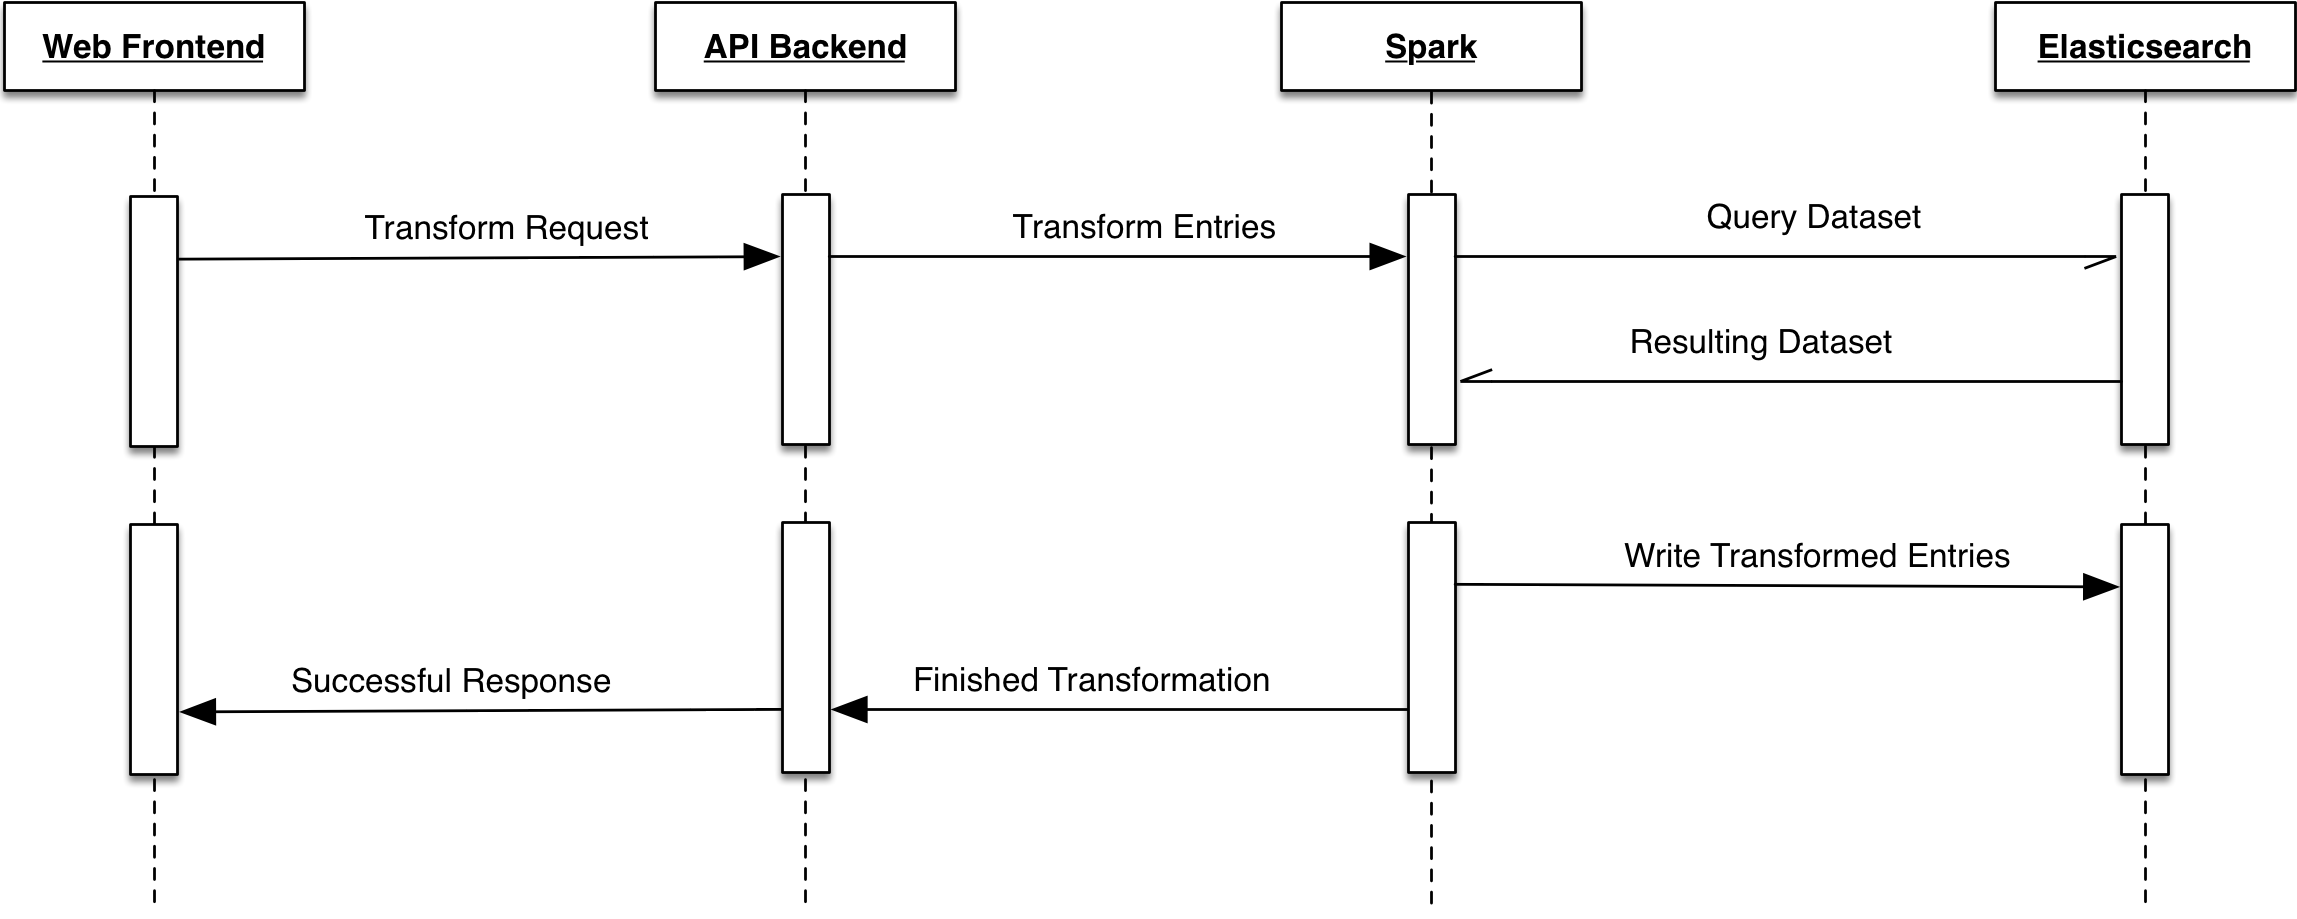
\includegraphics[width=1.05\textwidth]{figures/implementation/transformation-sequence}
  \caption{Sequence diagram showing the general data transformation flow.}
  \label{fig:transformation-sequence}
\end{figure}


\subsection{Features of TempMunger}

Our prototype\index{prototype} possesses the following main, high-level features regarding time-oriented\index{time-oriented} data, primarily focusing on visual-interactive\index{visual-interactive}, and particularly charting support:

\begin{itemize}
  \item \textbf{Transformations}\index{transformation}
  \begin{itemize}
    \item \textbf{Direct manipulation} via \gls{ui} controls
    \item \textbf{Cleaning} of missing and erroneous values
    \item \textbf{Normalization} concerning:
    \begin{itemize}
      \item Points in time
      \item Intervals
    \end{itemize}
    \item \textbf{Deletion} of rows
    \item \textbf{Merging} of columns
    \item \textbf{Formatting} cleanup
  \end{itemize}
  \item \textbf{Outlier detection}
  \item \textbf{Visual overview}
\end{itemize}

Furthermore, a more traditional \textbf{tabular editor} is available as known from spreadsheet applications like, most prominently, Microsoft Excel. Users are used to the underlying interaction metaphor and, consequently, it makes sense as a foundation to build upon.

\subsection{Transformations}

A central part of the approach\index{approach} is transformation\index{transformation} of time-oriented\index{time-oriented} data.
Generally, this is being achieved by making use of Apache Spark processing of Elasticsearch data.
As mentioned above, transformation\index{transformation} operations include \textbf{cleaning}, \textbf{normalization}, and \textbf{merging}.
Figure~\ref{fig:transformation-sequence} is presenting the general underlying flow via a sequence diagram.


\subsection{Outlier Detection}

Our prototype\index{prototype} applies some \gls{ml} techniques for its temporal outlier detection component.


\subsubsection{K-Means Clustering}

This is a popular algorithm of \emph{unsupervised learning}, i.e., \gls{ml} which does not rely on manual classification input, but rather classifies recognized patterns autonomously.

Formula~\ref{eq:k-means} represents its core principle, partitioning real vectorized observations $x$ into $k$ class cluster sets $S$ by calculating mean distances to respective centers ($\mu$ being the mean of points in $S_i$), generally computationally applying statistics\index{statistics} to pattern recognition:

\begin{equation}
\argmin_{S} \sum_{i=1}^{k} \sum_{x \in S_{i}} \|x - \mu_{i}\|^{2}
\label{eq:k-means}
\end{equation}

The following explains how this can be used for anomaly respectively outlier detection.

\subsubsection{Outlier Detection Usage}

The algorithm applied for our outlier detection component, basically, works as depicted in Algorithm~\ref{alg:temp-outlier-detection}.

A peculiar detail of our approach\index{approach} is that there is no dedicated test set of ``new'' data.
This is due to the fact there is only one dataset available at a time with no additional data coming in to extend it.
Thus, after training on a randomly split set, the whole dataset is used as test set, in the end, leading to overall satisfactory results.
Moreover, we are limiting the number of classes to be clustered to two.
Hence, our simple heuristic for determining an outlier class is to take the one of the two with fewer members.
When there is only one class, it is assumed no outliers could be detected.

\subsubsection{The Temporal Dimension}

Our use case revolves around finding outliers in time-oriented\index{time-oriented} data.
Figure~\ref{fig:outlier-detection-sequence} shows the basic, related flow with a sequence diagram.
In principle, we are using all time-oriented\index{time-oriented} data values available in the dataset at hand for vectorizing the observations to be input to clustering.
Therefore, the corresponding epoch millisecond values are used and if a certain value cannot be parsed it is substituted with a max. large number.
Consequently, missing and erroneous values are likely to be subsequently tagged as outliers as well.

\newpage


\begin{algorithm}
  \KwIn{A set of temporal field names $\varphi$ and a corresponding RDD (dataset) $\delta$}
  \KwOut{An RDD $\pi$ consisting of pairs of document ID to cluster class value}
  Vectorize dataset $\delta$ using field values via $\varphi$, see conditional (ll. 2-6)\;
  \eIf{a field value can be parsed as temporal}{
    Use its epoch milli value\;
  }{
    Use max. large number\;
  }
  Get training set $\tau$ from dataset $\delta$ via random split of $0.9 : 0.1$\;
  Create predictive model $\mu$ from vectors $\vec{x}$ of training set $\tau$\;
  $\to$ $k$-$means$ clustering yielding $2$ classes in $20$ iterations and $3$ parallel runs\;
  Predict points of dataset $\delta$ via model $\mu$, resulting in RDD $\pi$, see loop (ll. 11-14)\;
  \For{each point $\in$ dataset $\delta$}
  {
    Predict cluster class via model $\mu$\;
    Add result to RDD $\pi$\ via map op;
  }
  \Return{RDD $\pi$;}
  \caption{Temporal Outlier Detection}
  \label{alg:temp-outlier-detection}
\end{algorithm}

To further describe key points of the algorithm:\\
First, the dataset at hand is vectorized in order to enable applying it for clustering.
Then, a training set is generated from it via random split.
After that, a predictive model is created from the training set.
Afterwards, the dataset at hand is predictively clustered via model.
Finally, potential outliers are determined via aforementioned, simple heuristic.

\begin{figure}[h]
  \centering
  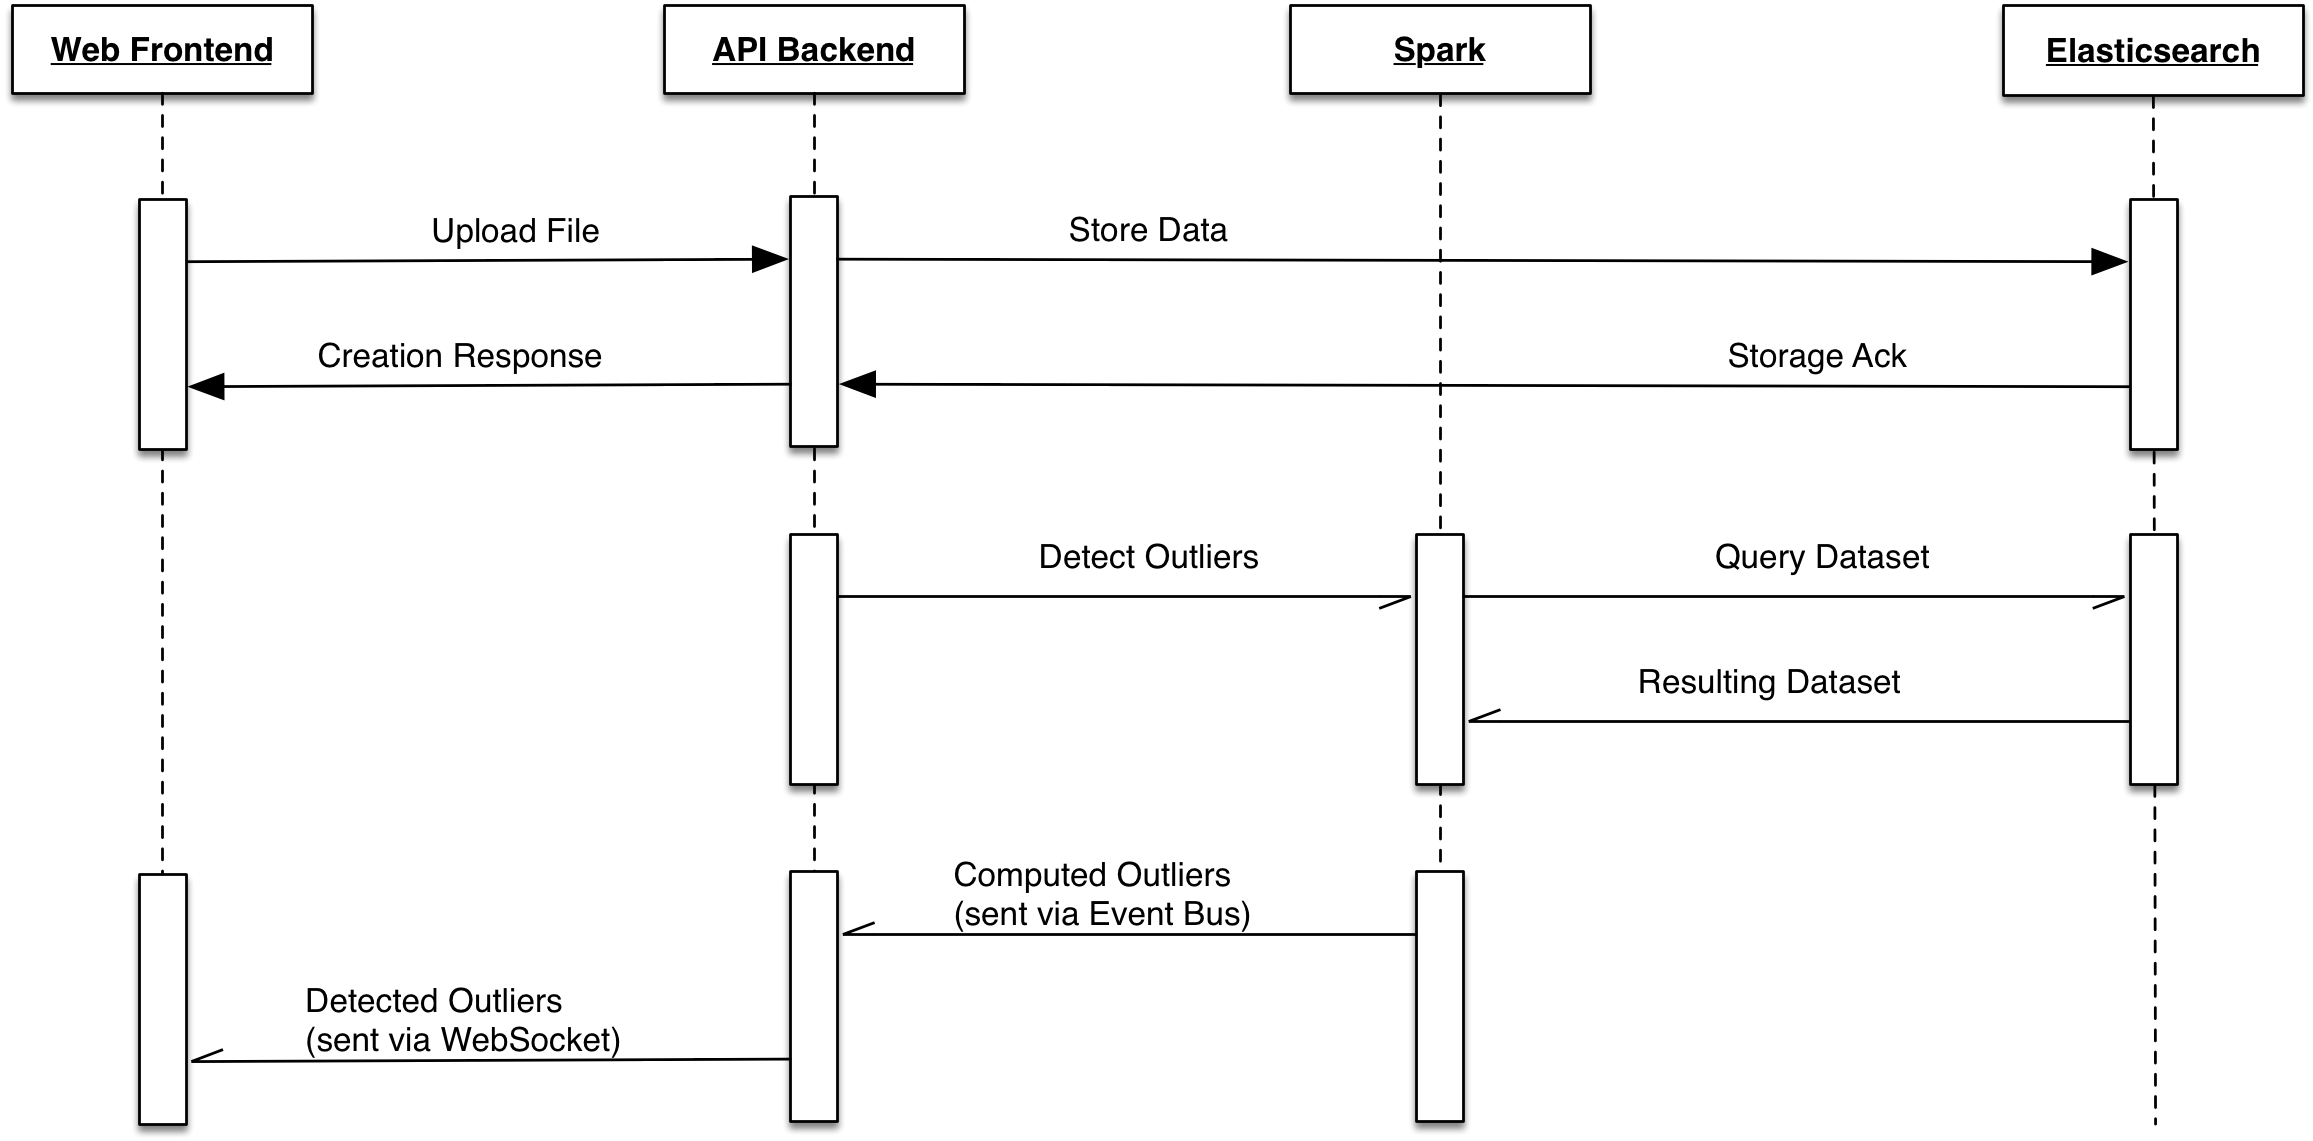
\includegraphics[width=1.025\textwidth]{figures/implementation/outlier-detection-sequence}
  \caption{Sequence diagram showing the general outlier detection on upload flow.}
  \label{fig:outlier-detection-sequence}
\end{figure}

\newpage


\subsection{Workflows and Screens}

In this section, workflows plus related screens of the implemented prototype\index{prototype} are described and explained.
Moreover, special emphasis is laid upon the reasoning behind the chosen path of the solution.


\subsubsection{Upload and Outlier Detection}

Initially, the user will want to upload some dataset to the application.
Therefore, a modal upload dialog is pretty conveniently reachable in the upper right corner of the screen.
This button is also visually especially noticeable via its peculiar coloring.
The upload dialog itself is designed\index{design} as simple as possible (see Figure~\ref{fig:screenshot-upload}).
One can either simply drag \& drop a file to it or select one via \gls{fs} dialog.
As soon as a file is selected, the upload begins and is indicating its progress via related animations.
In general, whenever data is being fetched respectively backend requests are issued, a spinning wheel effect is shown in the upper left corner of the screen.
When uploading is finished the dialog disappears and the user is free to interact with the data.

\begin{figure}[h]
  \centering
  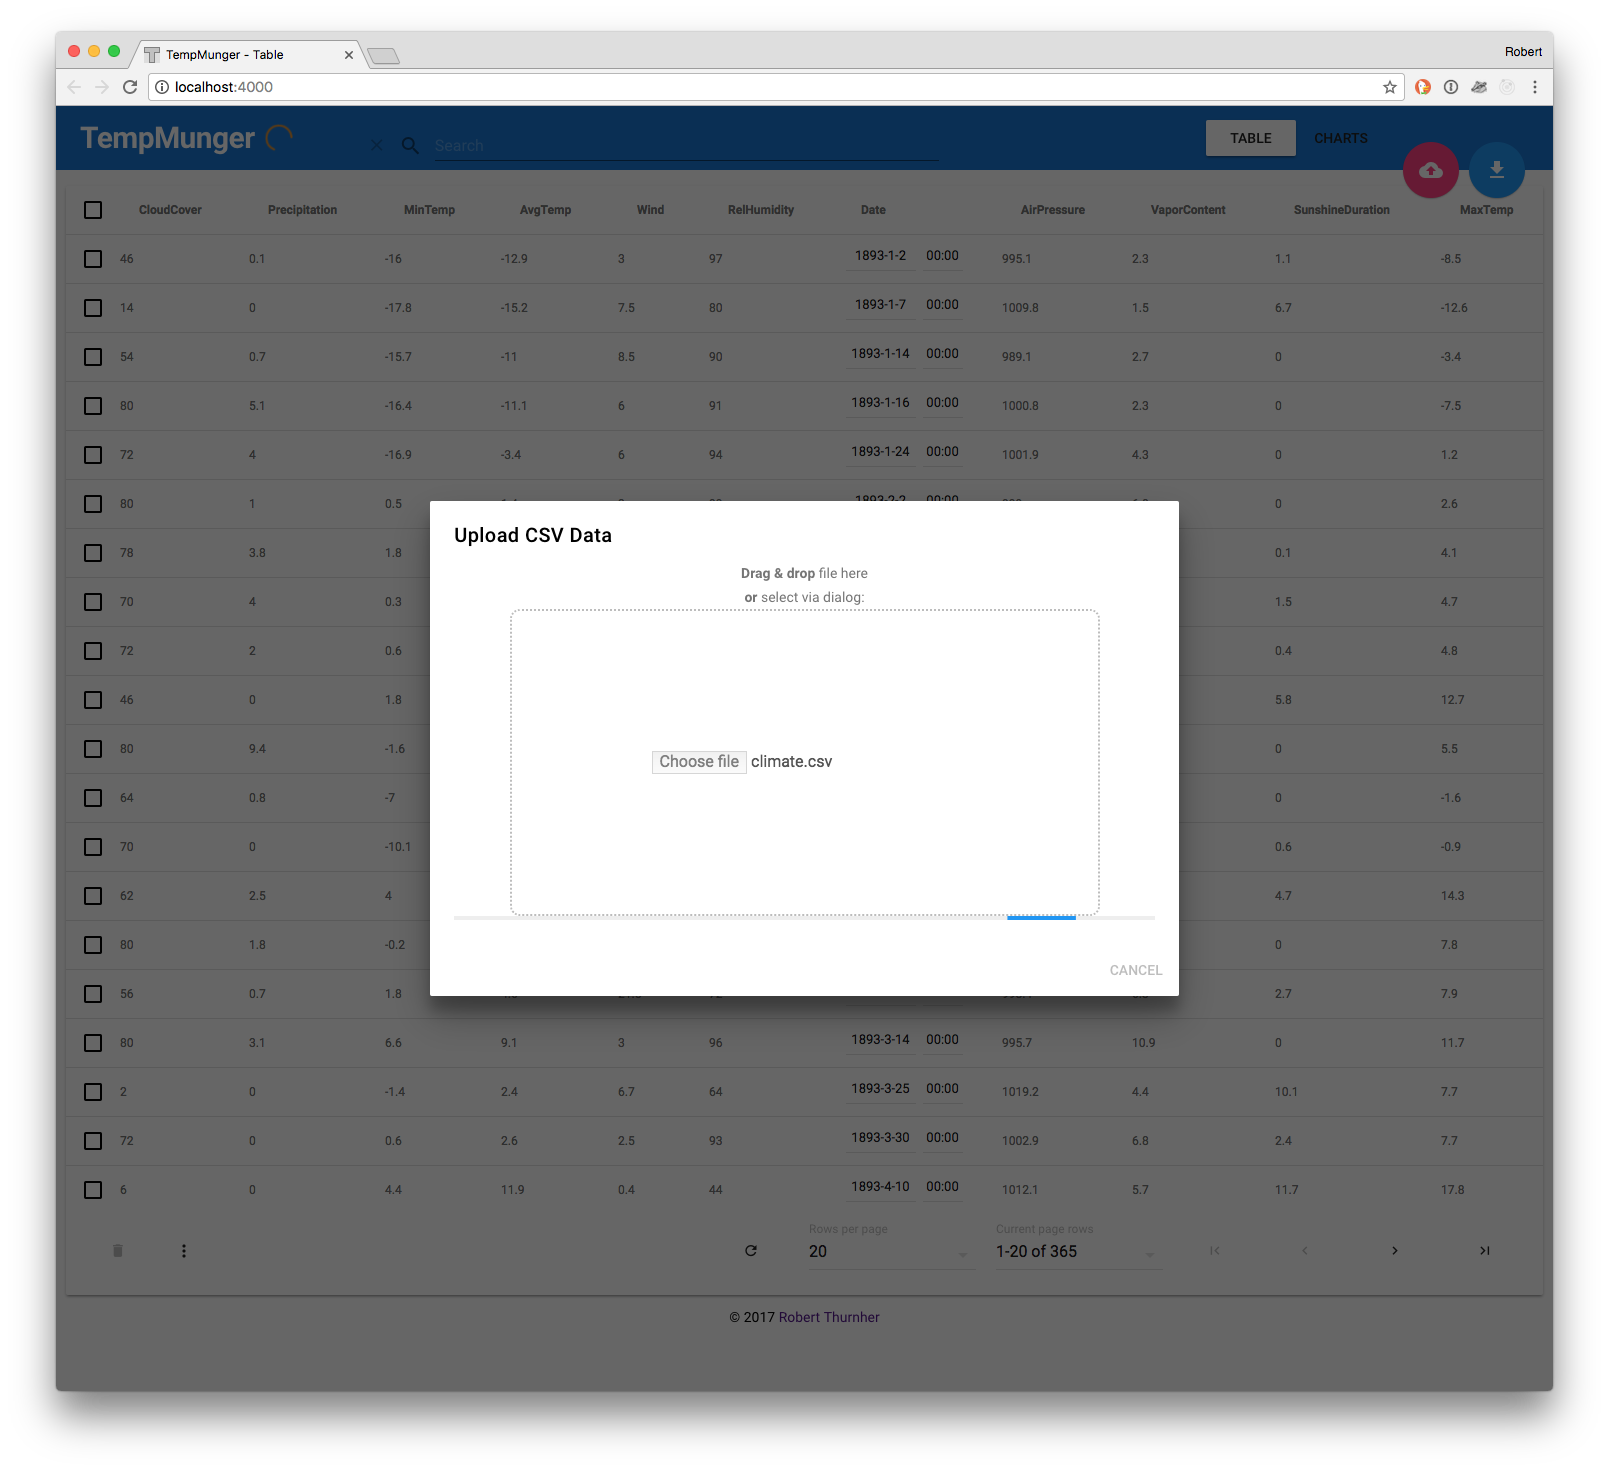
\includegraphics[width=1.0\textwidth]{figures/implementation/screenshot-upload}
  \caption{Screenshot showing upload with corresponding modal dialog and animated effects regarding progress indication.}
  \label{fig:screenshot-upload}
\end{figure}

As presented more from its technical side before, when uploading, an outlier detection mechanism is triggered.
On finished processing, the user is shown an according notification.
This message is sent as desktop browser respectively system notification\footnote{\textcolor{blue}{\href{https://developer.mozilla.org/en-US/docs/Web/API/Notifications_API}{developer.mozilla.org/en-US/docs/Web/API/Notifications\_API}}} (see Figure~\ref{fig:screenshot-notification}) as well as within the application itself as some sort of flashing notification from the bottom of the screen (see Figure~\ref{fig:screenshot-table-editor}).
The former stay around while the latter disappear.

When clicking a notification, an action is triggered filtering all dataset entries down to the potentially outlying ones.
The user may then proceed to act upon accordingly, having the potential outliers ready in sight and at her/his fingertips.
Presence of this filter is indicated via a chip-like control at the top of the screen (see Figure~\ref{fig:screenshot-search+filtering}).
It can be removed simply by clicking.

\begin{figure}[h]
  \centering
  
\includegraphics[width=0.66\textwidth]{figures/implementation/screenshot-notification}
  \caption{Screenshot showing desktop browser respectively system notification for interactive suggestive outlier detection indication.}
  \label{fig:screenshot-notification}
\end{figure}

\subsubsection{Table Editor}

A central component of the \gls{ui} is the table editor view page (see Figure~\ref{fig:screenshot-table-editor}).

There the user can directly manipulate the data at hand via editing corresponding cells.
Pagination controls at the bottom of the page allow for convenient paging through the data.
Page size can be adjusted as well as a particular page selected via related dropdowns.
Multi-row deletion is supported via selection checkboxes at the left side of the table.
It is possible to select rows one-by-one or (de)select all at once.
The connected deletion button is located at the bottom left of the table.

\subsubsection{Date/Time Picker}

Date and time picker \gls{ui} controls are used whenever an editable input field contains time-oriented\index{time-oriented} data.

The date picker allows the user to choose a date in an interactive way with the metaphor of a more traditional calendar (see Figure~\ref{fig:screenshot-date-picker}).
Whereas the time picker uses the metaphor of an analog clock for choosing a time value (see Figure~\ref{fig:screenshot-time-picker}).

\begin{figure}[h]
  \centering
  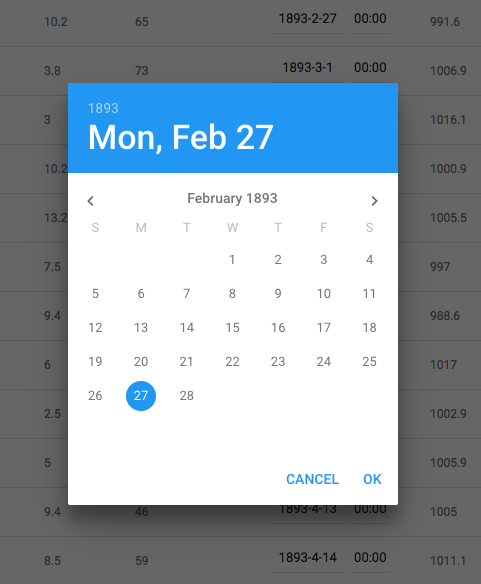
\includegraphics[width=0.525\textwidth]{figures/implementation/screenshot-date-picker}
  \caption{Screenshot showing exemplary modal date picker control with its calendar interaction metaphor.}
  \label{fig:screenshot-date-picker}
\end{figure}

\begin{figure}[h]
  \centering
  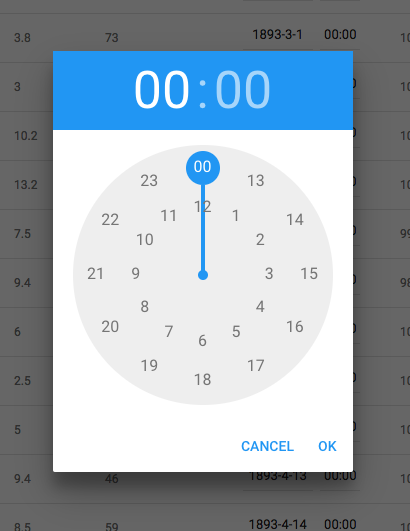
\includegraphics[width=0.525\textwidth]{figures/implementation/screenshot-time-picker}
  \caption{Screenshot showing exemplary modal time picker control with its clock interaction metaphor.}
  \label{fig:screenshot-time-picker}
\end{figure}

Both of these controls are commonly used throughout the application and normally in cooperation.
For instance, the table editor employs the controls for editing temporal column row values.

\subsubsection{Search and Filtering}

There are various ways in which filtering, slicing, and dicing the dataset is supported:

\begin{itemize}
  \item First of all, a search box is placed quite prominently at the top of the screen.
This enables the user to filter data down via full-text search.
  \item Additionally, as mentioned above, multiple rows can be selected.
Filter presence is indicated via aforementioned chip-like control.
The filter affects displayed data in the charts view page as well.
  \item Rows can be sorted by column values in ascending or descending order.
For this a simple click on the respective column header suffices.
  \item Furthermore, on the table view page there is a pagination available, see above.
\end{itemize}

All of these filtering options are working together correspondingly (see Figure~\ref{fig:screenshot-search+filtering}).

\subsubsection{Missing Values Cleanup}

It is possible to clean up missing and/or erroneous values via a modal dialog overlay (see Figure~\ref{fig:screenshot-missing-values}).
Missing respectively erroneous in this context means that the values were not able to be parsed as temporal.
The dialog can be accessed from the table editor view page at the bottom left via menu.
Its menu option is only available when the currently loaded dataset contains at least one time-oriented\index{time-oriented} data field.

On the modal dialog there is a dropdown to select one of the available temporal fields.
Below it there is a horizontal multi-bar chart consisting of two bars.
One of them represents all rows, and the other, missing values.
The former are colored in a neutral gray, while the latter are colored orange.
Consequently, a visual emphasis on the missing values is established.
The bars can be displayed grouped or stacked to get a better feel of the quantities at hand.
Below the chart there is a date and a time picker control for choosing a target value to fill the missing values with.
It is originally set to the average value of all values of the respective field (excluding missing ones).
At the bottom of the dialog there are action buttons to either apply the fill operation as described or to delete all rows with missing values.

\begin{figure}[h]
  \centering
  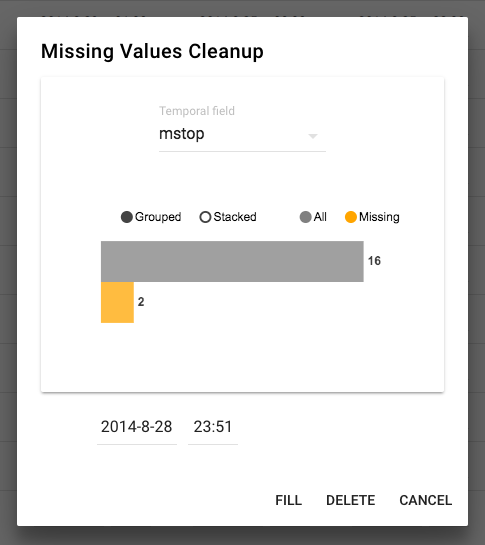
\includegraphics[width=0.7\textwidth]{figures/implementation/screenshot-missing-values}
  \caption{Screenshot showing missing values cleanup modal dialog overlay with charts.}
  \label{fig:screenshot-missing-values}
\end{figure}

\subsubsection{Temporal Normalization}

There are, basically, two types of temporal normalization operations supported by the prototype\index{prototype} -- this is not representing normalization in the strictest mathematical sense:

\begin{enumerate}
  \item Transform\index{transformation} all values within a certain timespan or at a certain point in time to a specified date/time
  \item Transform\index{transformation} all values within a certain interval, effectively ``moving'' them in time
\end{enumerate}

The former can be accessed either by clicking on a calendar heatmap or a distribution chart bar item on the charts view page (see Figure~\ref{fig:screenshot-charts-dialog}).
It is generally showing the selected timespan or point in time and enabling the user to set a target value via date and time picker controls for transforming\index{transformation} all affected values to.
Alternatively, the user can choose to delete all rows within the temporal selection.

\begin{figure}[h]
  \centering
  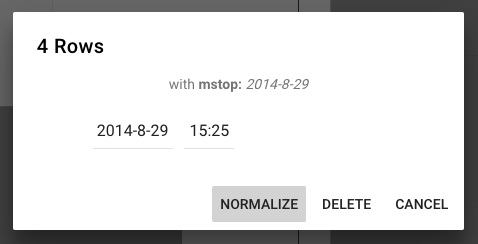
\includegraphics[width=0.66\textwidth]{figures/implementation/screenshot-charts-dialog}
  \caption{Screenshot showing charts page modal dialog on bar or heatmap item click.}
  \label{fig:screenshot-charts-dialog}
\end{figure}

The latter is accessible via a dedicated menu item at the bottom of the table editor view page, next to the one for missing values cleanup (see Figure~\ref{fig:screenshot-normalization}).
There the user can select a temporal field and interval, offering year or month.
When month is chosen at max. 10 bars in a chart are displayed each representing a month.
When year is chosen the bars represent years.
This is an aggregated view visualizing distribution of values with respective amounts sorted in descending order.
Again, bars are colored in a neutral gray. When selecting a bar its color changes to black, signalizing the selection. Plus, temporal input field controls show up. In the case of year interval being selected, there is a numeric text input for a target year.
In the case of month interval selection, there is additionally a dropdown with the 12 months of a year.
In addition to transforming\index{transformation} values accordingly, the user can also choose to delete selected rows instead.

\begin{figure}[h]
  \centering
  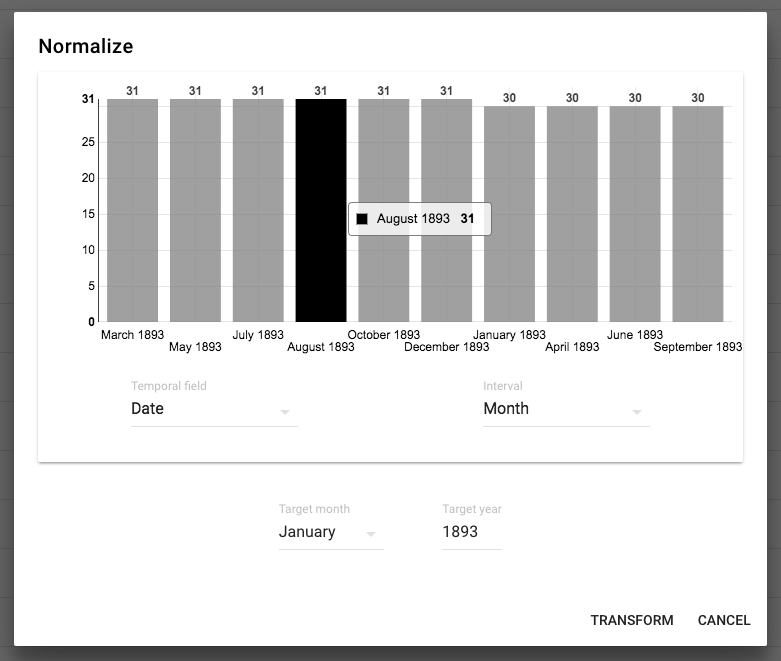
\includegraphics[width=1.0\textwidth]{figures/implementation/screenshot-normalization}
  \caption{Screenshot showing interval normalization modal dialog overlay with interactive bar charts and controls.}
  \label{fig:screenshot-normalization}
\end{figure}

\subsubsection{Table Column Merging}

It is possible to merge time-oriented\index{time-oriented} data columns via drag \& drop of table editor headers (see Figure~\ref{fig:screenshot-column-merge}).
Only columns containing temporal data are able to be drag \& dropped.
Interaction flow, generally, works as follows:

\begin{itemize}
  \item When starting to drag a header, possible drop targets (i.e., other temporal column headers) are highlighted in light yellow background color
  \item When dragging over a possible drop target, the hovered column header is highlighted in light green to signalize the drop possibility to the user
  \item When dragging over a non-temporal column header, it is highlighted in light orange color indicating that it is not a possible drop target
  \item When the user drops the dragged header on a possible target, a corresponding modal dialog overlay opens
\end{itemize}

This dialog asks the user to confirm merging columns as specified or cancel otherwise.
Merging, basically, works in the following way:

\begin{itemize}
  \item If both column values contain a temporal one, an average of these is used for the merged value
  \item If only one column value contains a temporal one, the missing one is substituted with the existing
  \item If both column values contain missing ones, an overall average of all values of the two columns is used
\end{itemize}

An alternative implementation could have given the user options to choose in a more fine-grained way.
Yet, we have found that these sensible defaults should make sense in many cases and the user can still apply further refinements of the column data after merge, if desired.
Naturally, on finished operation, the merge respectively drag source column is removed.

\begin{figure}[h]
  \centering
  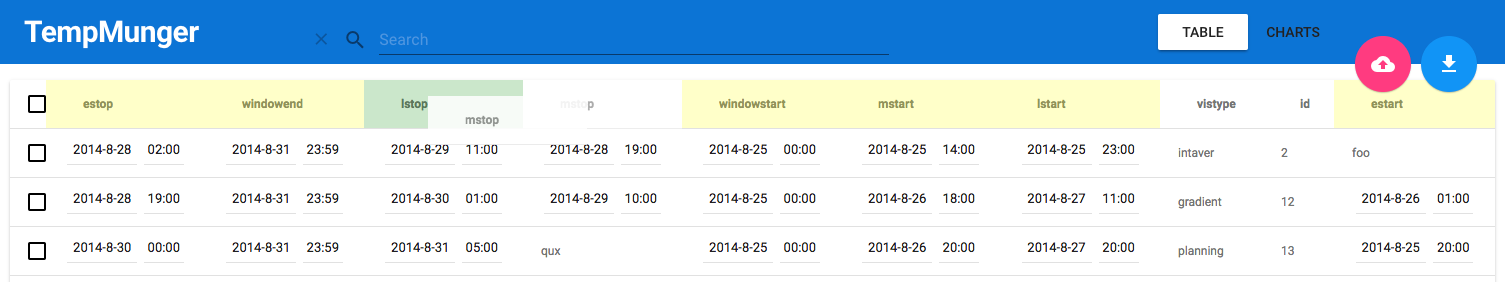
\includegraphics[width=1.0\textwidth]{figures/implementation/screenshot-column-merge}
  \caption{Screenshot showing table column merging via drag \& drop interaction.}
  \label{fig:screenshot-column-merge}
\end{figure}

\subsubsection{Charts Page}

The central \gls{ui} component regarding charts is kind of a dashboard page (see Figure~\ref{fig:screenshot-charts-page}).

When there are time-oriented\index{time-oriented} fields present in the respective dataset, it is headed by an interactive calendar heatmap visualization. It gives the user the opportunity to understand the temporal dimension of the data as well as transforming\index{transformation} it. Temporal fields can be selected via dropdown.

In any case and below there are two distribution bar charts next to each other.
These charts enable the user to get a grasp of the present data, plus transforming\index{transformation} it, too.
Again, fields can be selected via dropdown.

\subsubsection{Calendar Heatmap}

The calendar heatmap visualization, generally, allows four temporal scales \\(see Figure~\ref{fig:screenshot-calendar-heatmap}):

\begin{enumerate}
  \item Year
  \item Month (default)
  \item Week
  \item Day
\end{enumerate}

\begin{figure}[h]
  \centering
  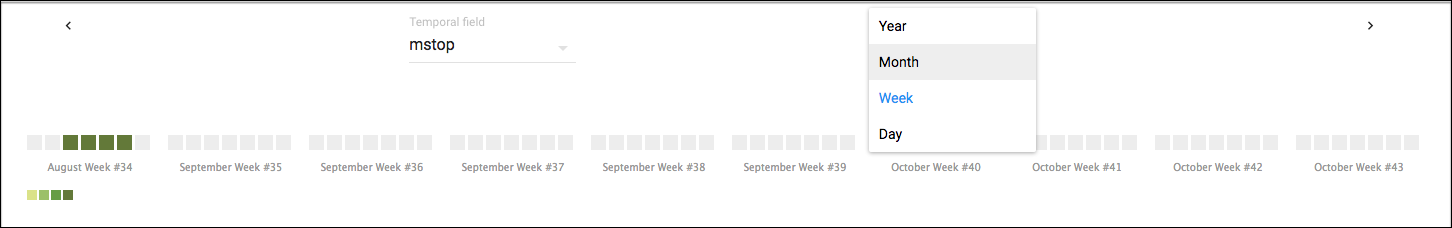
\includegraphics[width=1.0\textwidth]{figures/implementation/screenshot-calendar-heatmap}
  \caption{Screenshot showing calendar heatmap visualization with interactive controls.}
  \label{fig:screenshot-calendar-heatmap}
\end{figure}

Depending on the chosen scale the calendar view adjusts accordingly.
So, for instance, in the case of month scale, it is showing days of each month as boxes.
Furthermore, a color scale from gray via light to dark green indicates the amount of dataset entries associated with a certain temporal value represented by such a calendar item box.
On click of an item box, a modal dialog is shown, giving the user transform\index{transformation} options.

\subsubsection{Distribution Charts}

The two distribution bar charts can be seen as some sort of histogram visualizations, showing top aggregations.
They are mainly pointed at enabling the user to understand general data distribution qualities of the dataset at hand.
Plus, making it possible to easily compare these (see Figure~\ref{fig:screenshot-bar-charts}).
Again, clicking a bar opens a modal dialog for further interactive transformation\index{transformation} operations, like deletion or time-oriented\index{time-oriented} normalization.

\subsubsection{Export}

At the end of the day, the user wants to export the wrangled\index{wrangle} data.
Therefore, a button is quite prominently placed in the upper right corner of the application.
When there is no time-oriented\index{time-oriented} data included, a button click simply initiates a \textsc{CSV} file export download.
Otherwise, a modal dialog overlay is presented first.
This dialog lets the user choose a format to apply to all time-oriented\index{time-oriented} data of the to be exported dataset (see Figure~\ref{fig:screenshot-export-dialog}).

\begin{figure}[h]
  \centering
  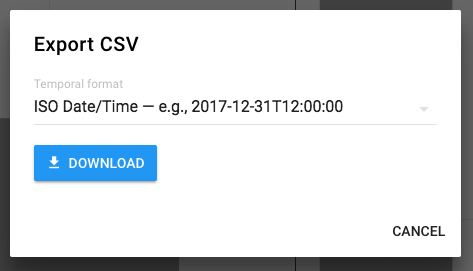
\includegraphics[width=0.66\textwidth]{figures/implementation/screenshot-export-dialog}
  \caption{Screenshot showing modal export dialog with temporal format dropdown.}
  \label{fig:screenshot-export-dialog}
\end{figure}

Three options are implemented and, consequently, available:

\begin{enumerate}
  \item \textsc{ISO}\footnote{\textcolor{blue}{\href{http://www.iso.org/iso/iso8601}{www.iso.org/iso/iso8601}}} date/time (e.g., \emph{2017-12-31T12:00:00})
  \item \textsc{ISO} date (e.g., \emph{2017-12-31})
  \item Epoch millis (e.g., \emph{1485037113334})
\end{enumerate}

Since all time-oriented\index{time-oriented} data is formatted on export in a unified way as well as uniformly stored in \gls{utc}/\gls{gmt} timezone on upload, there is no need to support formatting during previous editing and transformation\index{transformation} interactions.

\begin{sidewaysfigure}[h]
  \centering
  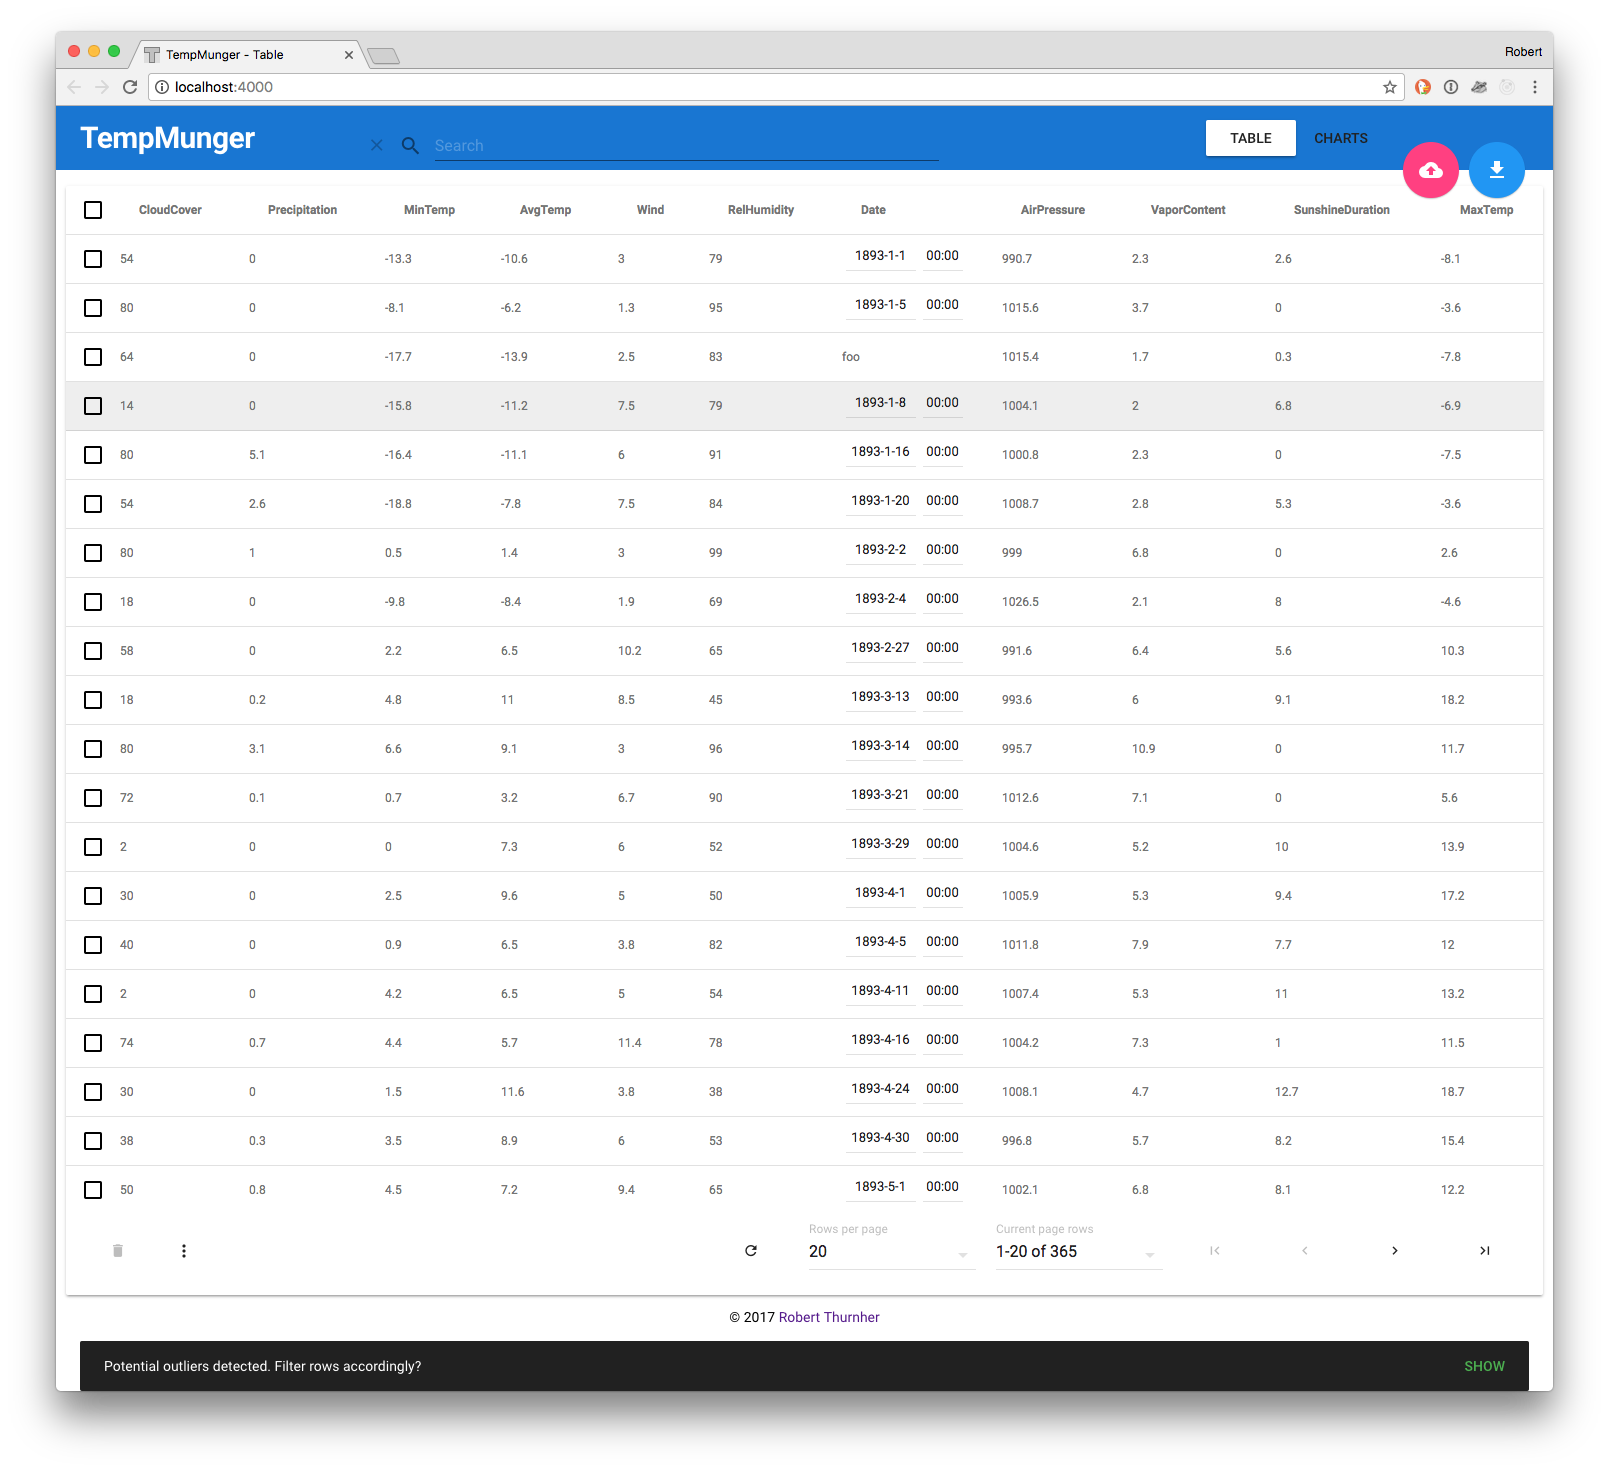
\includegraphics[width=0.9\textwidth]{figures/implementation/screenshot-table-editor}
  \caption{Screenshot showing table editor respectively main page including outlier detection info alert.}
  \label{fig:screenshot-table-editor}
\end{sidewaysfigure}

\begin{sidewaysfigure}[h]
  \centering
  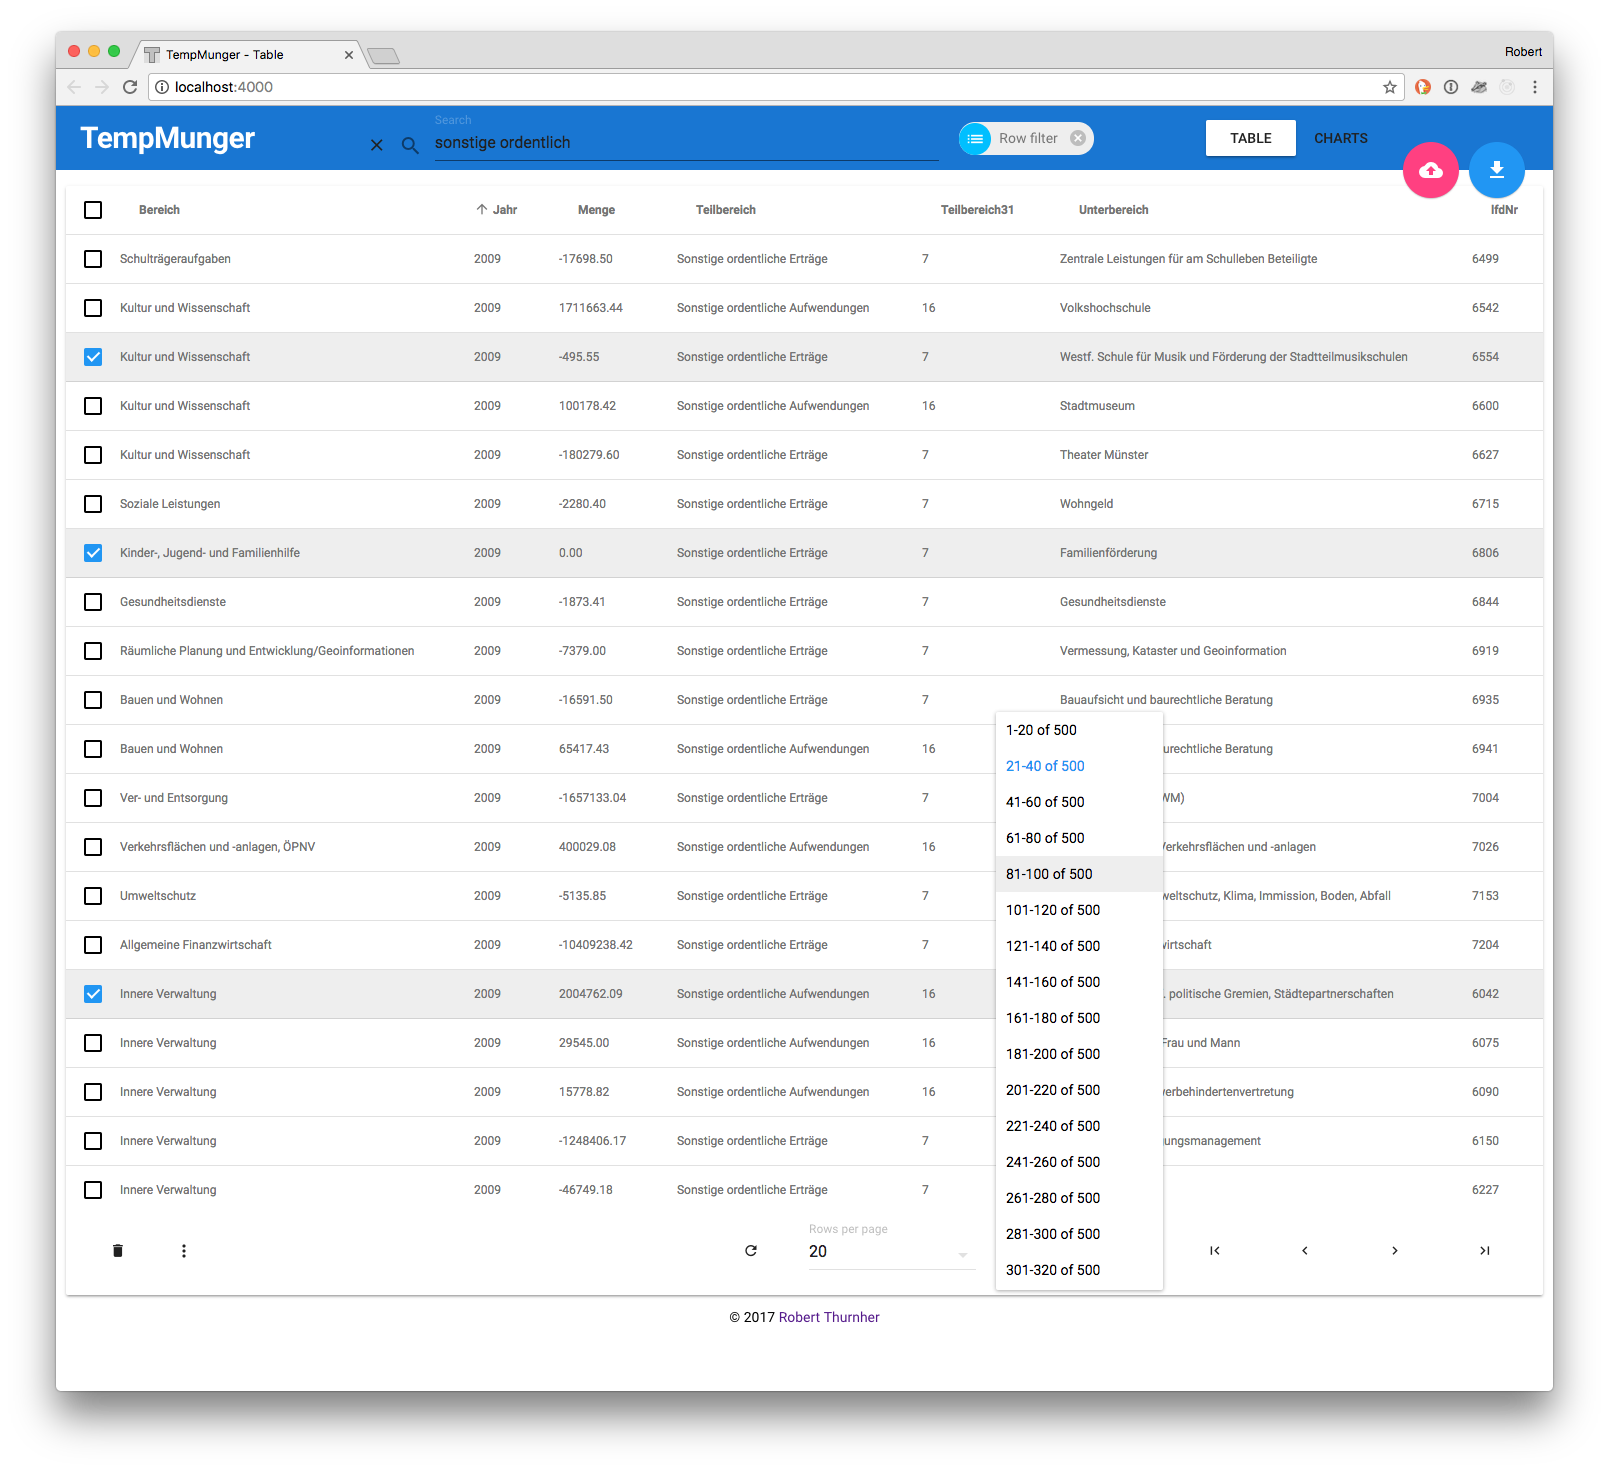
\includegraphics[width=0.9\textwidth]{figures/implementation/screenshot-search+filtering}
  \caption{Screenshot showing various navigational, search, and filtering options with table editor view.}
  \label{fig:screenshot-search+filtering}
\end{sidewaysfigure}

\begin{figure}[h]
  \centering
  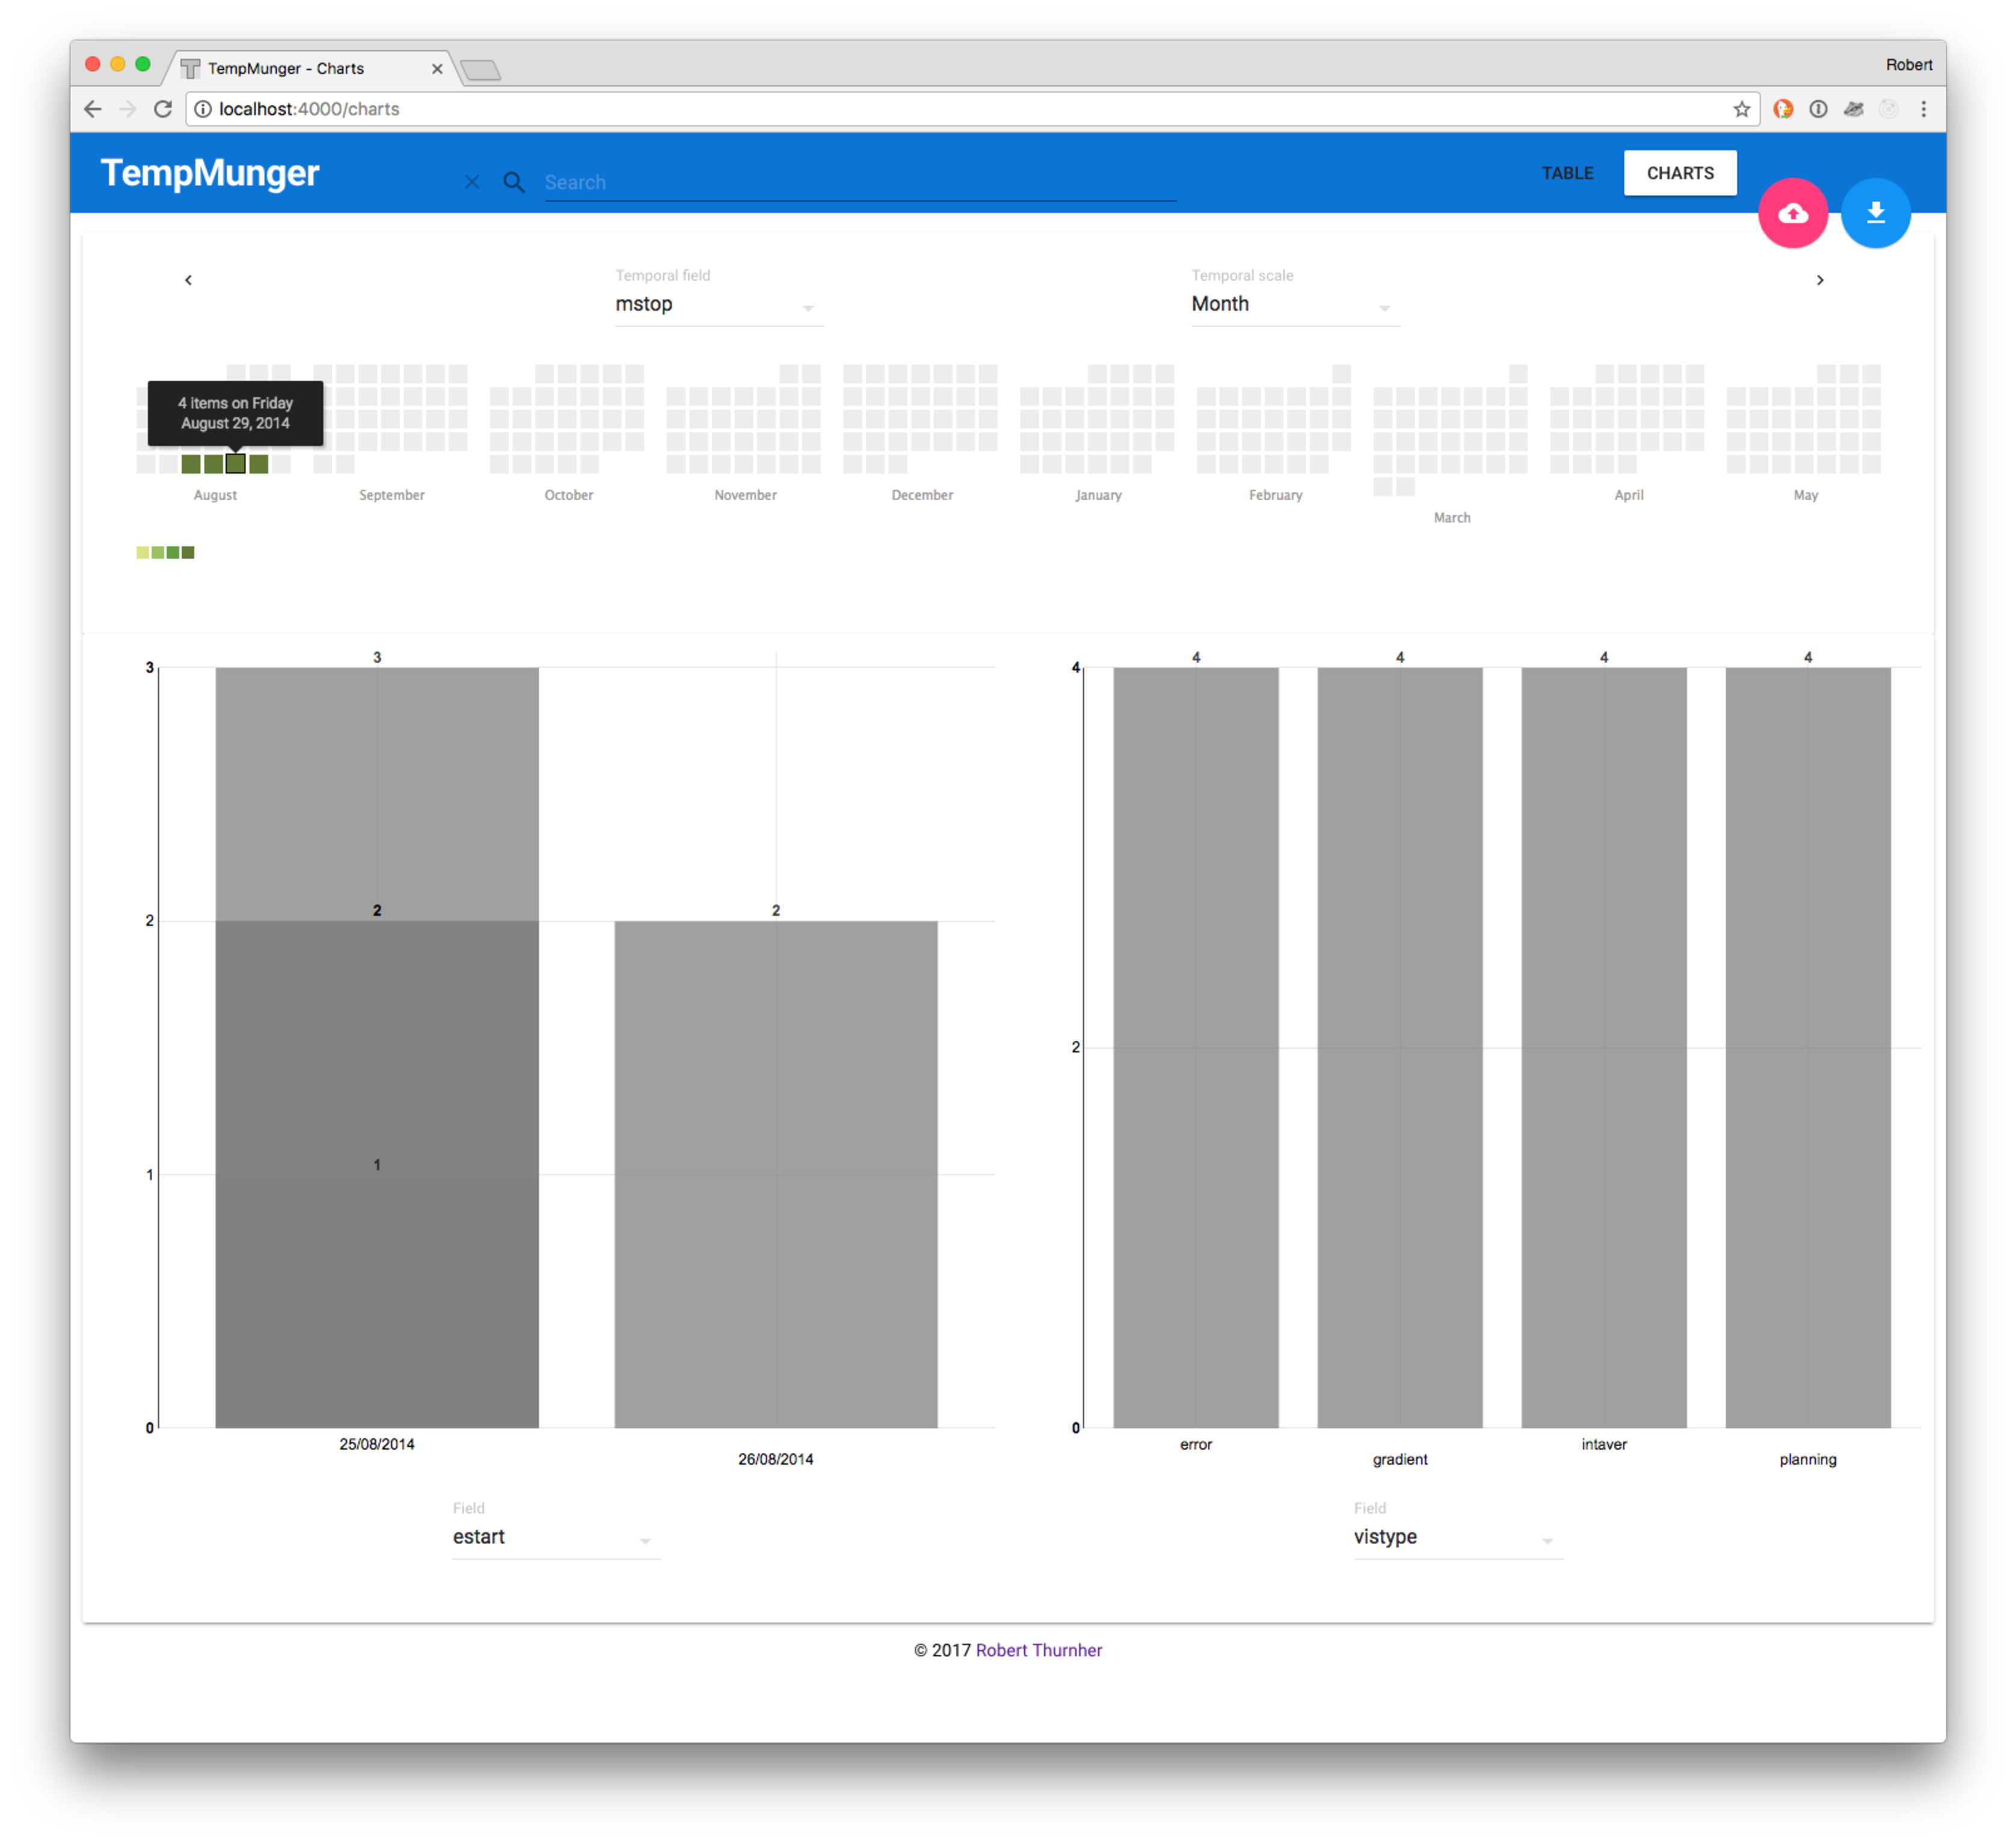
\includegraphics[width=0.9\textwidth]{figures/implementation/screenshot-charts-page}
  \caption{Screenshot of charts page with calendar heatmap, offering visual overview.}
  \label{fig:screenshot-charts-page}
\end{figure}

\begin{figure}[h]
  \centering
  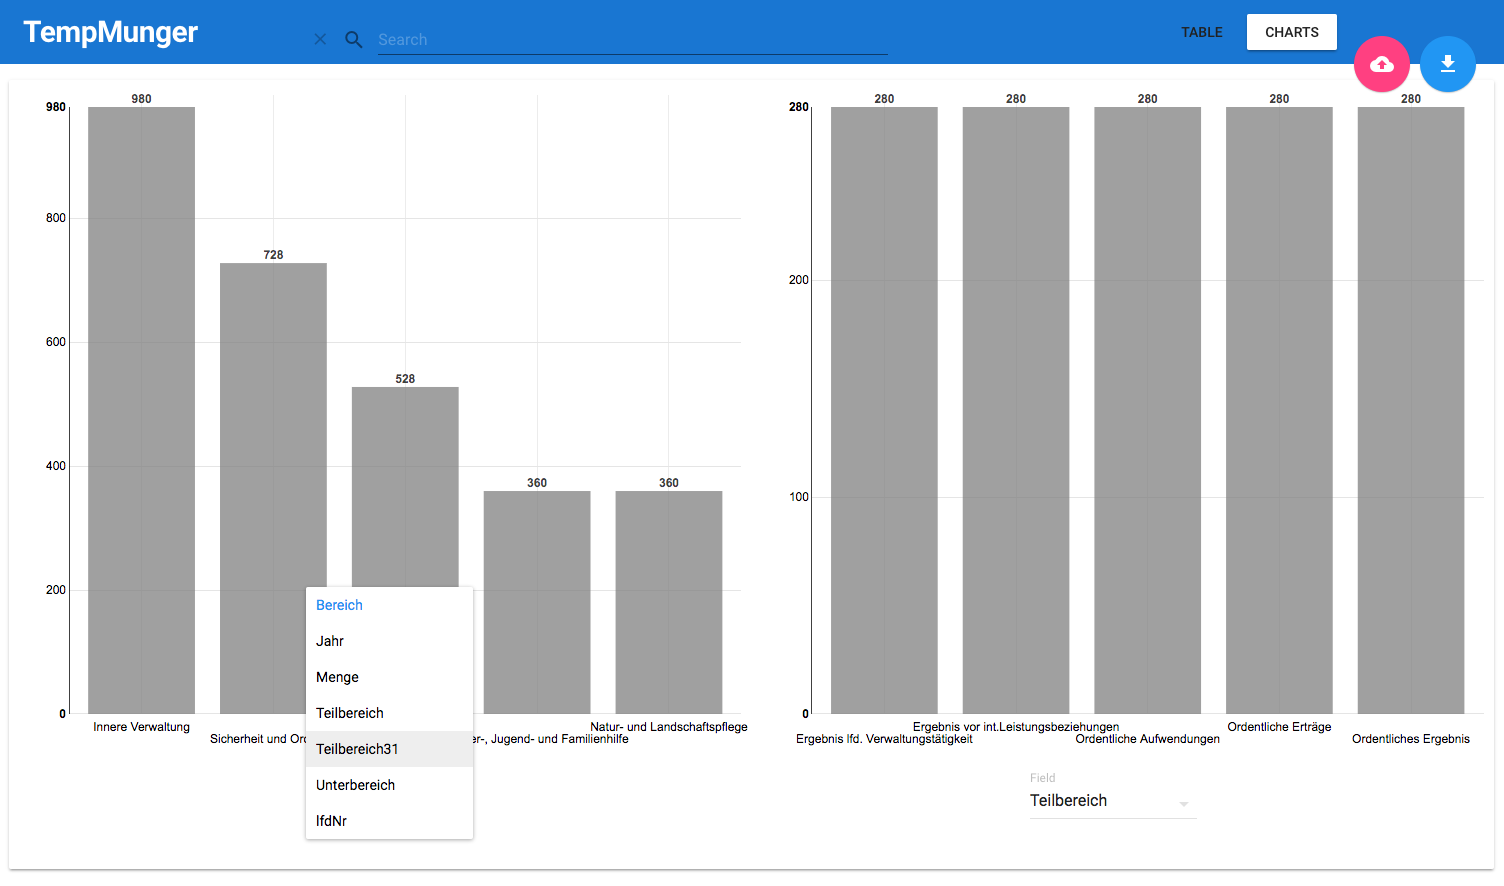
\includegraphics[width=0.777\textwidth]{figures/implementation/screenshot-bar-charts}
  \caption{Screenshot showing distribution bar charts with their dropdown controls.}
  \label{fig:screenshot-bar-charts}
\end{figure}


\section{Qualitative Evaluation} \label{sec:qualitative-evaluation}

Eventually, the results had to be evaluated.
For that matter, we have employed two well-known approaches\index{approach} and tools from the domain of usability engineering.
Both of which are introduced and extensively explained in \cite{Nielsen1993}:

\begin{enumerate}
  \item \textbf{Heuristic evaluation}
  \item \textbf{User/usability tests}
\end{enumerate}

The former basically means that an application and especially its \gls{ui} is being evaluated by a group of usability experts, step by step examining the to be evaluated system.
According to Holzinger~\cite{Holzinger2005} three to five usability experts are sufficient for this type of evaluation.
Therefore, we have conducted an heuristic evaluation with three experts.
Each of the experts should, further, evaluate independently from the others.
The evaluation is generally based on heuristics related to usability.
The classic ones as described by Nielsen~\cite{Nielsen1993} are:

\begin{itemize}
  \item \emph{Visibility of system status}
  \item \emph{Match between system and the real world}
  \item \emph{User control and freedom}
  \item \emph{Consistency and standards}
  \item \emph{Error prevention}
  \item \emph{Recognition rather than recall}
  \item \emph{Flexibility and efficiency of use}
  \item \emph{Aesthetic and minimalist design\index{design}}
  \item \emph{Help users recognize, diagnose, and recover from errors}
  \item \emph{Help and documentation}
\end{itemize}

Forsell and Johansson~\cite{Forsell2010} identified heuristic sets which are especially useful when dealing with applications in the realm of \gls{infovis}.
Therefore, we are adding the following:

\begin{itemize}
  \item \emph{Information coding}
  \item \emph{Spatial organization}
  \item \emph{Remove the extraneous}
\end{itemize}

For the evaluation itself each expert is asked to perform a given set of tasks.
Before that, a session going through the application and \gls{ui} in general is conducted.
An observer is present at the evaluation, who is familiar with the application and can be asked related questions.
The respective evaluator should note all issues.
At the end, found results are gathered and summarized.

These are the tasks we have established for our evaluation:

\begin{enumerate}
  \item Upload a dataset using a given \textsc{CSV} file
  \item Edit time-oriented\index{time-oriented} data via table editor
  \item Find potential outliers in the given dataset
  \item Identify missing respectively erroneous values
  \item Fill these with actual temporal values and/or delete their entries
  \item Normalize all entries in a certain month, moving them to another one
  \item Move all entries on a specific day to another point in time
  \item Delete all entries within a certain timespan or on a certain date
  \item Merge time-oriented\index{time-oriented} data columns on the table editor view page
  \item Export data as \textsc{CSV}, choosing a format for time-oriented\index{time-oriented} values
\end{enumerate}

User or usability tests, on the other hand, are usually performed in some sort of lab environment.
That is, users are given tasks to execute for reaching certain goals with the application and are being observed while doing so.
Typically, the test participants should be actually potential users.
We have performed such tests with two users, thus, in addition to the previous heuristic evaluation which we have conducted with three different usability and visualization experts.
The users of the user/usability tests were given the same tasks to perform as the experts from heuristic evaluation before.
Meanwhile testing and particularly afterwards they were interviewed regarding their experience, impressions, and opinions.
Finally, we have analyzed and abstracted connected findings.

The main questions all such user test participants as well as heuristic evaluation ones were asked:

\begin{enumerate}
  \item What is your overall impression?
  \item What are the strengths of TempMunger?
  \item What are the shortcomings of TempMunger?
  \item Do you believe TempMunger can be useful for you?
  \item If not, what do you think is needed to make it so?
\end{enumerate}

Combined results of the heuristic evaluation and user tests are as follows, listing found issues and linking them to their respective related, violated heuristics:

\begin{enumerate}
  \item Insufficient immediate and intuitive visual feedback regarding performed actions, e.g., on missing values cleanup ($\rightarrow$ \emph{visibility of system status})
  \item Findability of modal dialogs for missing values cleanup and interval-based normalization is suboptimal ($\rightarrow$ \emph{spatial organization})
  \item Separation of the two normalization dialogs as well as connected semantics are not intuitive and could be refined ($\rightarrow$ \emph{consistency and standards})
  \item Granularity of temporal scale is partially incomplete ($\rightarrow$ \emph{user control and freedom})
  \item Temporal scale coloring in calendar heatmap visualization is sometimes misleading ($\rightarrow$ \emph{information coding})
  \item No dedicated highlighting of concrete outlier values, for instance, via corresponding coloring ($\rightarrow$ \emph{recognition rather than recall})
  \item Outlier detection action could be made repeatable via button ($\rightarrow$ \emph{flexibility and efficiency of use})
  \item Merging operation could be made more useful by offering options and information regarding algorithm ($\rightarrow$ \emph{user control and freedom})
  \item Distribution charts for exploratory comparison on charts page could be enhanced, e.g., by adding drilling functionality ($\rightarrow$ \emph{information coding})
  \item In some places labels could be added to make controls and respective intention clearer ($\rightarrow$ \emph{remove the extraneous})
  \item Missing values cleanup dialog visualization could be refined, for instance, by making stacked charts view the default ($\rightarrow$ \emph{information coding})
  \item Calendar heatmap visualization could be enabled to make use of drag \& drop interaction ($\rightarrow$ \emph{flexibility and efficiency of use})
  \item Time-oriented\index{time-oriented} data could be displayed localized in controls and related input fields ($\rightarrow$ \emph{information coding})
  \item Multi-delete action button could be moved to the top of screen or made contextual ($\rightarrow$ \emph{user control and freedom})
  \item Large number of columns could lead to displaying glitches on the table editor view ($\rightarrow$ \emph{spatial organization})
\end{enumerate}

The heuristic category which was noted most often is \emph{information coding}, followed by \emph{user control and freedom}.
After that, \emph{spatial organization} as well as \emph{flexibility and efficiency of use} both got an equal amount of mentions.
Other categories scored only once each.
Hence, one can deduct a relative order concerning areas for possible improvements accordingly.

Generally, the approach\index{approach} and prototype\index{prototype} was perceived positively and as moving into the right direction.
In its current state it was rather seen as a nice proof of concept.
To make it a real-world applicable tool it would mainly need to be completed regarding coverage of data types, apart from its focus on time-oriented\index{time-oriented} one now.
Additionally, the currently provided set of transformation operations should be completed.
Furthermore, the present chart visualizations could be refined and including additional ones was encouraged.
Most frequently, possibly dotted, line charts were referred to in the context of time series data visualization as a potentially useful addition.
A central issue to address is scalability of the visualizations, also in regard to data granularity.

Aspects of our prototype most praised were the general visual design, the good visually interactive\index{visual-interactive} overview offered with charting aid, and smoothness regarding \gls{ux}.
On the other hand, usability was also one of the most controversially discussed topics as it is by its nature a highly subjective and opinionated one.
Moreover, an area for future work identified to be desirable would be to provide more transformation\index{transformation} suggestions interactively, in a proactive way.
Also, additional focus could be laid on further increasing interactive data filtering and drilling capabilities.
An interesting idea mentioned was that it could also be useful to some users being able to export visualizations in addition to the raw \textsc{CSV} data which is currently downloadable.
Finally, a feedback given by one of the test participants, which we especially appreciate, was \emph{``it does what it's supposed to do''}.

Regarding our interview questions more concretely and in detail:
answers to the first question connected to overall impression can be summarized as TempMunger being seen as a nice tool for the use case of working with time-oriented data visual-interactively\index{visual-interactive}.
Concerning strengths, most commonly pleasantness of general design, \gls{ux}, and quality of present visualizations were mentioned.
The interactive calendar heatmap as well as histogram-like bar chart visualizations were mostly seen as basically fitting for their purpose of conveniently visualizing data distribution focusing on time-oriented aspects and, therefore, useful.
Weaknesses were mainly identified to be related to lack of completeness of supported transformation operations and visualizations.
Thus, mainly coverage of varied specificity was found to have to be completed in order to make TempMunger a really versatile tool, outgrowing being merely a research prototype.

Further discussion of open issues and future work can be found in the conclusion sections following this one.
